% Created by tikzDevice version 0.12.6 on 2025-02-11 19:53:24
% !TEX encoding = UTF-8 Unicode
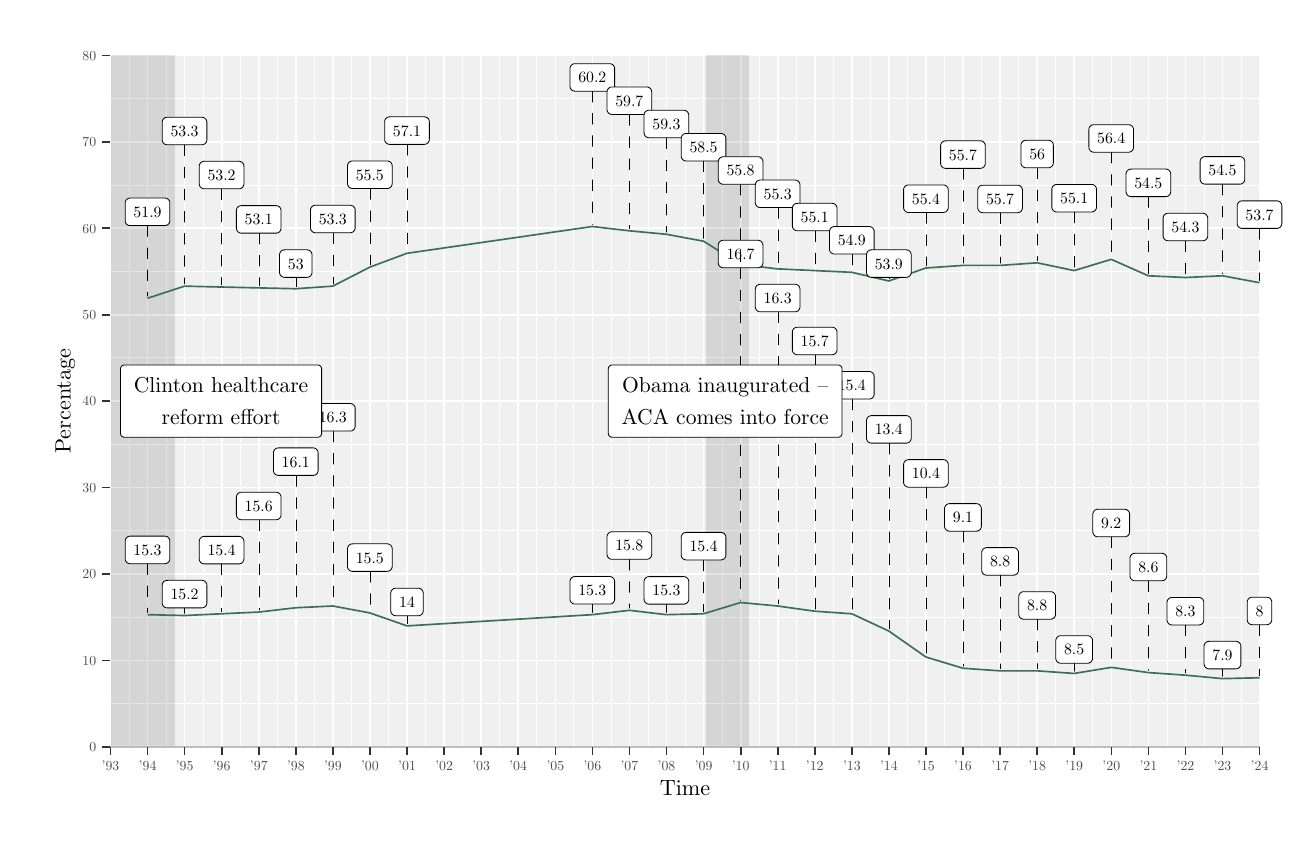
\begin{tikzpicture}[x=1pt,y=1pt]
\definecolor{fillColor}{RGB}{255,255,255}
\path[use as bounding box,fill=fillColor,fill opacity=0.00] (0,0) rectangle (455.30,289.08);
\begin{scope}
\path[clip] (  0.00,  0.00) rectangle (455.30,289.08);
\definecolor{drawColor}{RGB}{255,255,255}
\definecolor{fillColor}{RGB}{255,255,255}

\path[draw=drawColor,line width= 0.6pt,line join=round,line cap=round,fill=fillColor] (  0.00,  0.00) rectangle (455.30,289.08);
\end{scope}
\begin{scope}
\path[clip] (  0.00,  0.00) rectangle (455.30,289.08);
\definecolor{fillColor}{gray}{0.94}

\path[fill=fillColor] ( 29.76, 29.18) rectangle (445.30,279.08);
\definecolor{drawColor}{RGB}{255,255,255}

\path[draw=drawColor,line width= 0.3pt,line join=round] ( 29.76, 44.80) --
	(445.30, 44.80);

\path[draw=drawColor,line width= 0.3pt,line join=round] ( 29.76, 76.04) --
	(445.30, 76.04);

\path[draw=drawColor,line width= 0.3pt,line join=round] ( 29.76,107.27) --
	(445.30,107.27);

\path[draw=drawColor,line width= 0.3pt,line join=round] ( 29.76,138.51) --
	(445.30,138.51);

\path[draw=drawColor,line width= 0.3pt,line join=round] ( 29.76,169.75) --
	(445.30,169.75);

\path[draw=drawColor,line width= 0.3pt,line join=round] ( 29.76,200.99) --
	(445.30,200.99);

\path[draw=drawColor,line width= 0.3pt,line join=round] ( 29.76,232.22) --
	(445.30,232.22);

\path[draw=drawColor,line width= 0.3pt,line join=round] ( 29.76,263.46) --
	(445.30,263.46);

\path[draw=drawColor,line width= 0.3pt,line join=round] ( 36.64, 29.18) --
	( 36.64,279.08);

\path[draw=drawColor,line width= 0.3pt,line join=round] ( 50.03, 29.18) --
	( 50.03,279.08);

\path[draw=drawColor,line width= 0.3pt,line join=round] ( 63.41, 29.18) --
	( 63.41,279.08);

\path[draw=drawColor,line width= 0.3pt,line join=round] ( 76.81, 29.18) --
	( 76.81,279.08);

\path[draw=drawColor,line width= 0.3pt,line join=round] ( 90.22, 29.18) --
	( 90.22,279.08);

\path[draw=drawColor,line width= 0.3pt,line join=round] (103.60, 29.18) --
	(103.60,279.08);

\path[draw=drawColor,line width= 0.3pt,line join=round] (116.99, 29.18) --
	(116.99,279.08);

\path[draw=drawColor,line width= 0.3pt,line join=round] (130.39, 29.18) --
	(130.39,279.08);

\path[draw=drawColor,line width= 0.3pt,line join=round] (143.80, 29.18) --
	(143.80,279.08);

\path[draw=drawColor,line width= 0.3pt,line join=round] (157.18, 29.18) --
	(157.18,279.08);

\path[draw=drawColor,line width= 0.3pt,line join=round] (170.57, 29.18) --
	(170.57,279.08);

\path[draw=drawColor,line width= 0.3pt,line join=round] (183.97, 29.18) --
	(183.97,279.08);

\path[draw=drawColor,line width= 0.3pt,line join=round] (197.38, 29.18) --
	(197.38,279.08);

\path[draw=drawColor,line width= 0.3pt,line join=round] (210.76, 29.18) --
	(210.76,279.08);

\path[draw=drawColor,line width= 0.3pt,line join=round] (224.15, 29.18) --
	(224.15,279.08);

\path[draw=drawColor,line width= 0.3pt,line join=round] (237.55, 29.18) --
	(237.55,279.08);

\path[draw=drawColor,line width= 0.3pt,line join=round] (250.95, 29.18) --
	(250.95,279.08);

\path[draw=drawColor,line width= 0.3pt,line join=round] (264.34, 29.18) --
	(264.34,279.08);

\path[draw=drawColor,line width= 0.3pt,line join=round] (277.73, 29.18) --
	(277.73,279.08);

\path[draw=drawColor,line width= 0.3pt,line join=round] (291.13, 29.18) --
	(291.13,279.08);

\path[draw=drawColor,line width= 0.3pt,line join=round] (304.53, 29.18) --
	(304.53,279.08);

\path[draw=drawColor,line width= 0.3pt,line join=round] (317.92, 29.18) --
	(317.92,279.08);

\path[draw=drawColor,line width= 0.3pt,line join=round] (331.30, 29.18) --
	(331.30,279.08);

\path[draw=drawColor,line width= 0.3pt,line join=round] (344.71, 29.18) --
	(344.71,279.08);

\path[draw=drawColor,line width= 0.3pt,line join=round] (358.11, 29.18) --
	(358.11,279.08);

\path[draw=drawColor,line width= 0.3pt,line join=round] (371.50, 29.18) --
	(371.50,279.08);

\path[draw=drawColor,line width= 0.3pt,line join=round] (384.88, 29.18) --
	(384.88,279.08);

\path[draw=drawColor,line width= 0.3pt,line join=round] (398.29, 29.18) --
	(398.29,279.08);

\path[draw=drawColor,line width= 0.3pt,line join=round] (411.69, 29.18) --
	(411.69,279.08);

\path[draw=drawColor,line width= 0.3pt,line join=round] (425.08, 29.18) --
	(425.08,279.08);

\path[draw=drawColor,line width= 0.3pt,line join=round] (438.46, 29.18) --
	(438.46,279.08);

\path[draw=drawColor,line width= 0.6pt,line join=round] ( 29.76, 29.18) --
	(445.30, 29.18);

\path[draw=drawColor,line width= 0.6pt,line join=round] ( 29.76, 60.42) --
	(445.30, 60.42);

\path[draw=drawColor,line width= 0.6pt,line join=round] ( 29.76, 91.66) --
	(445.30, 91.66);

\path[draw=drawColor,line width= 0.6pt,line join=round] ( 29.76,122.89) --
	(445.30,122.89);

\path[draw=drawColor,line width= 0.6pt,line join=round] ( 29.76,154.13) --
	(445.30,154.13);

\path[draw=drawColor,line width= 0.6pt,line join=round] ( 29.76,185.37) --
	(445.30,185.37);

\path[draw=drawColor,line width= 0.6pt,line join=round] ( 29.76,216.61) --
	(445.30,216.61);

\path[draw=drawColor,line width= 0.6pt,line join=round] ( 29.76,247.84) --
	(445.30,247.84);

\path[draw=drawColor,line width= 0.6pt,line join=round] ( 29.76,279.08) --
	(445.30,279.08);

\path[draw=drawColor,line width= 0.6pt,line join=round] ( 29.95, 29.18) --
	( 29.95,279.08);

\path[draw=drawColor,line width= 0.6pt,line join=round] ( 43.33, 29.18) --
	( 43.33,279.08);

\path[draw=drawColor,line width= 0.6pt,line join=round] ( 56.72, 29.18) --
	( 56.72,279.08);

\path[draw=drawColor,line width= 0.6pt,line join=round] ( 70.10, 29.18) --
	( 70.10,279.08);

\path[draw=drawColor,line width= 0.6pt,line join=round] ( 83.53, 29.18) --
	( 83.53,279.08);

\path[draw=drawColor,line width= 0.6pt,line join=round] ( 96.91, 29.18) --
	( 96.91,279.08);

\path[draw=drawColor,line width= 0.6pt,line join=round] (110.30, 29.18) --
	(110.30,279.08);

\path[draw=drawColor,line width= 0.6pt,line join=round] (123.68, 29.18) --
	(123.68,279.08);

\path[draw=drawColor,line width= 0.6pt,line join=round] (137.10, 29.18) --
	(137.10,279.08);

\path[draw=drawColor,line width= 0.6pt,line join=round] (150.49, 29.18) --
	(150.49,279.08);

\path[draw=drawColor,line width= 0.6pt,line join=round] (163.88, 29.18) --
	(163.88,279.08);

\path[draw=drawColor,line width= 0.6pt,line join=round] (177.26, 29.18) --
	(177.26,279.08);

\path[draw=drawColor,line width= 0.6pt,line join=round] (190.68, 29.18) --
	(190.68,279.08);

\path[draw=drawColor,line width= 0.6pt,line join=round] (204.07, 29.18) --
	(204.07,279.08);

\path[draw=drawColor,line width= 0.6pt,line join=round] (217.45, 29.18) --
	(217.45,279.08);

\path[draw=drawColor,line width= 0.6pt,line join=round] (230.84, 29.18) --
	(230.84,279.08);

\path[draw=drawColor,line width= 0.6pt,line join=round] (244.26, 29.18) --
	(244.26,279.08);

\path[draw=drawColor,line width= 0.6pt,line join=round] (257.65, 29.18) --
	(257.65,279.08);

\path[draw=drawColor,line width= 0.6pt,line join=round] (271.03, 29.18) --
	(271.03,279.08);

\path[draw=drawColor,line width= 0.6pt,line join=round] (284.42, 29.18) --
	(284.42,279.08);

\path[draw=drawColor,line width= 0.6pt,line join=round] (297.84, 29.18) --
	(297.84,279.08);

\path[draw=drawColor,line width= 0.6pt,line join=round] (311.23, 29.18) --
	(311.23,279.08);

\path[draw=drawColor,line width= 0.6pt,line join=round] (324.61, 29.18) --
	(324.61,279.08);

\path[draw=drawColor,line width= 0.6pt,line join=round] (338.00, 29.18) --
	(338.00,279.08);

\path[draw=drawColor,line width= 0.6pt,line join=round] (351.42, 29.18) --
	(351.42,279.08);

\path[draw=drawColor,line width= 0.6pt,line join=round] (364.80, 29.18) --
	(364.80,279.08);

\path[draw=drawColor,line width= 0.6pt,line join=round] (378.19, 29.18) --
	(378.19,279.08);

\path[draw=drawColor,line width= 0.6pt,line join=round] (391.58, 29.18) --
	(391.58,279.08);

\path[draw=drawColor,line width= 0.6pt,line join=round] (405.00, 29.18) --
	(405.00,279.08);

\path[draw=drawColor,line width= 0.6pt,line join=round] (418.38, 29.18) --
	(418.38,279.08);

\path[draw=drawColor,line width= 0.6pt,line join=round] (431.77, 29.18) --
	(431.77,279.08);

\path[draw=drawColor,line width= 0.6pt,line join=round] (445.15, 29.18) --
	(445.15,279.08);
\definecolor{fillColor}{RGB}{190,190,190}

\path[fill=fillColor,fill opacity=0.01] ( 29.95, 29.18) rectangle ( 53.16,279.08);

\path[fill=fillColor,fill opacity=0.01] ( 29.95, 29.18) rectangle ( 53.16,279.08);

\path[fill=fillColor,fill opacity=0.01] ( 29.95, 29.18) rectangle ( 53.16,279.08);

\path[fill=fillColor,fill opacity=0.01] ( 29.95, 29.18) rectangle ( 53.16,279.08);

\path[fill=fillColor,fill opacity=0.01] ( 29.95, 29.18) rectangle ( 53.16,279.08);

\path[fill=fillColor,fill opacity=0.01] ( 29.95, 29.18) rectangle ( 53.16,279.08);

\path[fill=fillColor,fill opacity=0.01] ( 29.95, 29.18) rectangle ( 53.16,279.08);

\path[fill=fillColor,fill opacity=0.01] ( 29.95, 29.18) rectangle ( 53.16,279.08);

\path[fill=fillColor,fill opacity=0.01] ( 29.95, 29.18) rectangle ( 53.16,279.08);

\path[fill=fillColor,fill opacity=0.01] ( 29.95, 29.18) rectangle ( 53.16,279.08);

\path[fill=fillColor,fill opacity=0.01] ( 29.95, 29.18) rectangle ( 53.16,279.08);

\path[fill=fillColor,fill opacity=0.01] ( 29.95, 29.18) rectangle ( 53.16,279.08);

\path[fill=fillColor,fill opacity=0.01] ( 29.95, 29.18) rectangle ( 53.16,279.08);

\path[fill=fillColor,fill opacity=0.01] ( 29.95, 29.18) rectangle ( 53.16,279.08);

\path[fill=fillColor,fill opacity=0.01] ( 29.95, 29.18) rectangle ( 53.16,279.08);

\path[fill=fillColor,fill opacity=0.01] ( 29.95, 29.18) rectangle ( 53.16,279.08);

\path[fill=fillColor,fill opacity=0.01] ( 29.95, 29.18) rectangle ( 53.16,279.08);

\path[fill=fillColor,fill opacity=0.01] ( 29.95, 29.18) rectangle ( 53.16,279.08);

\path[fill=fillColor,fill opacity=0.01] ( 29.95, 29.18) rectangle ( 53.16,279.08);

\path[fill=fillColor,fill opacity=0.01] ( 29.95, 29.18) rectangle ( 53.16,279.08);

\path[fill=fillColor,fill opacity=0.01] ( 29.95, 29.18) rectangle ( 53.16,279.08);

\path[fill=fillColor,fill opacity=0.01] ( 29.95, 29.18) rectangle ( 53.16,279.08);

\path[fill=fillColor,fill opacity=0.01] ( 29.95, 29.18) rectangle ( 53.16,279.08);

\path[fill=fillColor,fill opacity=0.01] ( 29.95, 29.18) rectangle ( 53.16,279.08);

\path[fill=fillColor,fill opacity=0.01] ( 29.95, 29.18) rectangle ( 53.16,279.08);

\path[fill=fillColor,fill opacity=0.01] ( 29.95, 29.18) rectangle ( 53.16,279.08);

\path[fill=fillColor,fill opacity=0.01] ( 29.95, 29.18) rectangle ( 53.16,279.08);

\path[fill=fillColor,fill opacity=0.01] (244.96, 29.18) rectangle (260.62,279.08);

\path[fill=fillColor,fill opacity=0.01] (244.96, 29.18) rectangle (260.62,279.08);

\path[fill=fillColor,fill opacity=0.01] (244.96, 29.18) rectangle (260.62,279.08);

\path[fill=fillColor,fill opacity=0.01] (244.96, 29.18) rectangle (260.62,279.08);

\path[fill=fillColor,fill opacity=0.01] (244.96, 29.18) rectangle (260.62,279.08);

\path[fill=fillColor,fill opacity=0.01] (244.96, 29.18) rectangle (260.62,279.08);

\path[fill=fillColor,fill opacity=0.01] (244.96, 29.18) rectangle (260.62,279.08);

\path[fill=fillColor,fill opacity=0.01] (244.96, 29.18) rectangle (260.62,279.08);

\path[fill=fillColor,fill opacity=0.01] (244.96, 29.18) rectangle (260.62,279.08);

\path[fill=fillColor,fill opacity=0.01] (244.96, 29.18) rectangle (260.62,279.08);

\path[fill=fillColor,fill opacity=0.01] (244.96, 29.18) rectangle (260.62,279.08);

\path[fill=fillColor,fill opacity=0.01] (244.96, 29.18) rectangle (260.62,279.08);

\path[fill=fillColor,fill opacity=0.01] (244.96, 29.18) rectangle (260.62,279.08);

\path[fill=fillColor,fill opacity=0.01] (244.96, 29.18) rectangle (260.62,279.08);

\path[fill=fillColor,fill opacity=0.01] (244.96, 29.18) rectangle (260.62,279.08);

\path[fill=fillColor,fill opacity=0.01] (244.96, 29.18) rectangle (260.62,279.08);

\path[fill=fillColor,fill opacity=0.01] (244.96, 29.18) rectangle (260.62,279.08);

\path[fill=fillColor,fill opacity=0.01] (244.96, 29.18) rectangle (260.62,279.08);

\path[fill=fillColor,fill opacity=0.01] (244.96, 29.18) rectangle (260.62,279.08);

\path[fill=fillColor,fill opacity=0.01] (244.96, 29.18) rectangle (260.62,279.08);

\path[fill=fillColor,fill opacity=0.01] (244.96, 29.18) rectangle (260.62,279.08);

\path[fill=fillColor,fill opacity=0.01] (244.96, 29.18) rectangle (260.62,279.08);

\path[fill=fillColor,fill opacity=0.01] (244.96, 29.18) rectangle (260.62,279.08);

\path[fill=fillColor,fill opacity=0.01] (244.96, 29.18) rectangle (260.62,279.08);

\path[fill=fillColor,fill opacity=0.01] (244.96, 29.18) rectangle (260.62,279.08);

\path[fill=fillColor,fill opacity=0.01] (244.96, 29.18) rectangle (260.62,279.08);

\path[fill=fillColor,fill opacity=0.01] (244.96, 29.18) rectangle (260.62,279.08);
\definecolor{drawColor}{RGB}{190,190,190}

\path[draw=drawColor,line width= 0.6pt,line join=round] ( 29.76, 29.18) -- (445.30, 29.18);
\definecolor{drawColor}{RGB}{60,113,79}

\path[draw=drawColor,line width= 0.6pt,line join=round] ( 43.30,191.30) --
	( 56.68,195.68) --
	( 70.07,195.36) --
	( 83.49,195.05) --
	( 96.87,194.74) --
	(110.26,195.68) --
	(123.65,202.55) --
	(137.07,207.55) --
	(204.03,217.23) --
	(217.42,215.67) --
	(230.80,214.42) --
	(244.23,211.92) --
	(257.61,203.49) --
	(271.00,201.92) --
	(284.38,201.30) --
	(297.80,200.67) --
	(311.19,197.55) --
	(324.57,202.24) --
	(337.96,203.17) --
	(351.38,203.17) --
	(364.77,204.11) --
	(378.15,201.30) --
	(391.54,205.36) --
	(404.96,199.42) --
	(418.35,198.80) --
	(431.73,199.42) --
	(445.12,196.93);

\path[draw=drawColor,line width= 0.6pt,line join=round] ( 43.30, 76.97) --
	( 56.68, 76.66) --
	( 70.07, 77.29) --
	( 83.49, 77.91) --
	( 96.87, 79.47) --
	(110.26, 80.10) --
	(123.65, 77.60) --
	(137.07, 72.91) --
	(204.03, 76.97) --
	(217.42, 78.54) --
	(230.80, 76.97) --
	(244.23, 77.29) --
	(257.61, 81.35) --
	(271.00, 80.10) --
	(284.38, 78.22) --
	(297.80, 77.29) --
	(311.19, 71.04) --
	(324.57, 61.67) --
	(337.96, 57.61) --
	(351.38, 56.67) --
	(364.77, 56.67) --
	(378.15, 55.73) --
	(391.54, 57.92) --
	(404.96, 56.04) --
	(418.35, 55.11) --
	(431.73, 53.86) --
	(445.12, 54.17);
\end{scope}
\begin{scope}
\path[clip] (  0.00,  0.00) rectangle (455.30,289.08);
\definecolor{drawColor}{RGB}{0,0,0}

\path[draw=drawColor,line width= 0.1pt,dash pattern=on 4pt off 4pt ,line join=round,line cap=round] ( 43.30, 95.39) -- ( 43.30, 77.70);

\path[draw=drawColor,line width= 0.1pt,dash pattern=on 4pt off 4pt ,line join=round,line cap=round] ( 56.68, 79.43) -- ( 56.68, 77.39);

\path[draw=drawColor,line width= 0.1pt,dash pattern=on 4pt off 4pt ,line join=round,line cap=round] ( 70.07, 95.31) -- ( 70.07, 78.01);

\path[draw=drawColor,line width= 0.1pt,dash pattern=on 4pt off 4pt ,line join=round,line cap=round] ( 83.49,111.27) -- ( 83.49, 78.64);

\path[draw=drawColor,line width= 0.1pt,dash pattern=on 4pt off 4pt ,line join=round,line cap=round] ( 96.87,127.29) -- ( 96.87, 80.20);

\path[draw=drawColor,line width= 0.1pt,dash pattern=on 4pt off 4pt ,line join=round,line cap=round] (110.26,143.31) -- (110.26, 80.82);

\path[draw=drawColor,line width= 0.1pt,dash pattern=on 4pt off 4pt ,line join=round,line cap=round] (123.65, 92.62) -- (123.65, 78.33);

\path[draw=drawColor,line width= 0.1pt,dash pattern=on 4pt off 4pt ,line join=round,line cap=round] (137.07, 76.59) -- (137.07, 73.64);

\path[draw=drawColor,line width= 0.1pt,dash pattern=on 4pt off 4pt ,line join=round,line cap=round] (204.03, 80.80) -- (204.03, 77.70);

\path[draw=drawColor,line width= 0.1pt,dash pattern=on 4pt off 4pt ,line join=round,line cap=round] (217.42, 96.97) -- (217.42, 79.26);

\path[draw=drawColor,line width= 0.1pt,dash pattern=on 4pt off 4pt ,line join=round,line cap=round] (230.80, 80.77) -- (230.80, 77.70);

\path[draw=drawColor,line width= 0.1pt,dash pattern=on 4pt off 4pt ,line join=round,line cap=round] (244.23, 96.75) -- (244.23, 78.01);

\path[draw=drawColor,line width= 0.1pt,dash pattern=on 4pt off 4pt ,line join=round,line cap=round] (257.61,202.32) -- (257.61, 82.07);

\path[draw=drawColor,line width= 0.1pt,dash pattern=on 4pt off 4pt ,line join=round,line cap=round] (271.00,186.41) -- (271.00, 80.82);

\path[draw=drawColor,line width= 0.1pt,dash pattern=on 4pt off 4pt ,line join=round,line cap=round] (284.38,170.90) -- (284.38, 78.95);

\path[draw=drawColor,line width= 0.1pt,dash pattern=on 4pt off 4pt ,line join=round,line cap=round] (297.80,154.89) -- (297.80, 78.01);

\path[draw=drawColor,line width= 0.1pt,dash pattern=on 4pt off 4pt ,line join=round,line cap=round] (311.19,138.94) -- (311.19, 71.77);

\path[draw=drawColor,line width= 0.1pt,dash pattern=on 4pt off 4pt ,line join=round,line cap=round] (324.57,123.04) -- (324.57, 62.39);

\path[draw=drawColor,line width= 0.1pt,dash pattern=on 4pt off 4pt ,line join=round,line cap=round] (337.96,107.14) -- (337.96, 58.33);

\path[draw=drawColor,line width= 0.1pt,dash pattern=on 4pt off 4pt ,line join=round,line cap=round] (351.38, 91.24) -- (351.38, 57.40);

\path[draw=drawColor,line width= 0.1pt,dash pattern=on 4pt off 4pt ,line join=round,line cap=round] (364.77, 75.33) -- (364.77, 57.40);

\path[draw=drawColor,line width= 0.1pt,dash pattern=on 4pt off 4pt ,line join=round,line cap=round] (378.15, 59.42) -- (378.15, 56.46);

\path[draw=drawColor,line width= 0.1pt,dash pattern=on 4pt off 4pt ,line join=round,line cap=round] (391.54,105.10) -- (391.54, 58.65);

\path[draw=drawColor,line width= 0.1pt,dash pattern=on 4pt off 4pt ,line join=round,line cap=round] (404.96, 89.21) -- (404.96, 56.77);

\path[draw=drawColor,line width= 0.1pt,dash pattern=on 4pt off 4pt ,line join=round,line cap=round] (418.35, 73.26) -- (418.35, 55.83);

\path[draw=drawColor,line width= 0.1pt,dash pattern=on 4pt off 4pt ,line join=round,line cap=round] (431.73, 57.39) -- (431.73, 54.59);

\path[draw=drawColor,line width= 0.1pt,dash pattern=on 4pt off 4pt ,line join=round,line cap=round] (445.12, 73.35) -- (445.12, 54.90);
\definecolor{fillColor}{RGB}{255,255,255}

\path[draw=drawColor,line width= 0.3pt,line join=round,line cap=round,fill=fillColor] ( 37.03, 95.39) --
	( 49.56, 95.39) --
	( 49.49, 95.39) --
	( 49.78, 95.41) --
	( 50.06, 95.46) --
	( 50.33, 95.57) --
	( 50.58, 95.71) --
	( 50.81, 95.90) --
	( 51.00, 96.11) --
	( 51.16, 96.36) --
	( 51.27, 96.63) --
	( 51.34, 96.91) --
	( 51.36, 97.20) --
	( 51.36, 97.20) --
	( 51.36,103.53) --
	( 51.36,103.53) --
	( 51.34,103.82) --
	( 51.27,104.10) --
	( 51.16,104.37) --
	( 51.00,104.61) --
	( 50.81,104.83) --
	( 50.58,105.02) --
	( 50.33,105.16) --
	( 50.06,105.26) --
	( 49.78,105.32) --
	( 49.56,105.34) --
	( 37.03,105.34) --
	( 37.25,105.32) --
	( 36.96,105.33) --
	( 36.67,105.30) --
	( 36.39,105.22) --
	( 36.13,105.09) --
	( 35.89,104.93) --
	( 35.68,104.73) --
	( 35.51,104.49) --
	( 35.37,104.24) --
	( 35.28,103.96) --
	( 35.23,103.67) --
	( 35.23,103.53) --
	( 35.23, 97.20) --
	( 35.23, 97.35) --
	( 35.23, 97.05) --
	( 35.28, 96.77) --
	( 35.37, 96.49) --
	( 35.51, 96.23) --
	( 35.68, 96.00) --
	( 35.89, 95.80) --
	( 36.13, 95.64) --
	( 36.39, 95.51) --
	( 36.67, 95.43) --
	( 36.96, 95.39) --
	cycle;
\end{scope}
\begin{scope}
\path[clip] (  0.00,  0.00) rectangle (455.30,289.08);
\definecolor{drawColor}{RGB}{0,0,0}

\node[text=drawColor,anchor=base,inner sep=0pt, outer sep=0pt, scale=  0.57] at ( 43.30, 98.40) {15.3};
\definecolor{fillColor}{RGB}{255,255,255}

\path[draw=drawColor,line width= 0.3pt,line join=round,line cap=round,fill=fillColor] ( 50.42, 79.43) --
	( 62.94, 79.43) --
	( 62.87, 79.44) --
	( 63.16, 79.45) --
	( 63.45, 79.51) --
	( 63.72, 79.61) --
	( 63.97, 79.75) --
	( 64.19, 79.94) --
	( 64.39, 80.16) --
	( 64.54, 80.40) --
	( 64.66, 80.67) --
	( 64.73, 80.95) --
	( 64.75, 81.24) --
	( 64.75, 81.24) --
	( 64.75, 87.57) --
	( 64.75, 87.57) --
	( 64.73, 87.86) --
	( 64.66, 88.14) --
	( 64.54, 88.41) --
	( 64.39, 88.65) --
	( 64.19, 88.87) --
	( 63.97, 89.06) --
	( 63.72, 89.20) --
	( 63.45, 89.31) --
	( 63.16, 89.36) --
	( 62.94, 89.38) --
	( 50.42, 89.38) --
	( 50.64, 89.36) --
	( 50.35, 89.37) --
	( 50.06, 89.34) --
	( 49.78, 89.26) --
	( 49.52, 89.13) --
	( 49.28, 88.97) --
	( 49.07, 88.77) --
	( 48.89, 88.54) --
	( 48.76, 88.28) --
	( 48.67, 88.00) --
	( 48.62, 87.71) --
	( 48.61, 87.57) --
	( 48.61, 81.24) --
	( 48.62, 81.39) --
	( 48.62, 81.10) --
	( 48.67, 80.81) --
	( 48.76, 80.53) --
	( 48.89, 80.28) --
	( 49.07, 80.04) --
	( 49.28, 79.84) --
	( 49.52, 79.68) --
	( 49.78, 79.55) --
	( 50.06, 79.47) --
	( 50.35, 79.44) --
	cycle;
\end{scope}
\begin{scope}
\path[clip] (  0.00,  0.00) rectangle (455.30,289.08);
\definecolor{drawColor}{RGB}{0,0,0}

\node[text=drawColor,anchor=base,inner sep=0pt, outer sep=0pt, scale=  0.57] at ( 56.68, 82.45) {15.2};
\definecolor{fillColor}{RGB}{255,255,255}

\path[draw=drawColor,line width= 0.3pt,line join=round,line cap=round,fill=fillColor] ( 63.80, 95.31) --
	( 76.33, 95.31) --
	( 76.26, 95.31) --
	( 76.55, 95.32) --
	( 76.83, 95.38) --
	( 77.10, 95.49) --
	( 77.36, 95.63) --
	( 77.58, 95.81) --
	( 77.77, 96.03) --
	( 77.93, 96.28) --
	( 78.04, 96.55) --
	( 78.11, 96.83) --
	( 78.14, 97.12) --
	( 78.14, 97.12) --
	( 78.14,103.45) --
	( 78.14,103.45) --
	( 78.11,103.74) --
	( 78.04,104.02) --
	( 77.93,104.29) --
	( 77.77,104.53) --
	( 77.58,104.75) --
	( 77.36,104.93) --
	( 77.10,105.08) --
	( 76.83,105.18) --
	( 76.55,105.24) --
	( 76.33,105.25) --
	( 63.80,105.25) --
	( 64.02,105.24) --
	( 63.73,105.25) --
	( 63.44,105.22) --
	( 63.16,105.14) --
	( 62.90,105.01) --
	( 62.66,104.85) --
	( 62.45,104.64) --
	( 62.28,104.41) --
	( 62.14,104.15) --
	( 62.05,103.88) --
	( 62.00,103.59) --
	( 62.00,103.45) --
	( 62.00, 97.12) --
	( 62.00, 97.26) --
	( 62.00, 96.97) --
	( 62.05, 96.69) --
	( 62.14, 96.41) --
	( 62.28, 96.15) --
	( 62.45, 95.92) --
	( 62.66, 95.72) --
	( 62.90, 95.55) --
	( 63.16, 95.43) --
	( 63.44, 95.35) --
	( 63.73, 95.31) --
	cycle;
\end{scope}
\begin{scope}
\path[clip] (  0.00,  0.00) rectangle (455.30,289.08);
\definecolor{drawColor}{RGB}{0,0,0}

\node[text=drawColor,anchor=base,inner sep=0pt, outer sep=0pt, scale=  0.57] at ( 70.07, 98.32) {15.4};
\definecolor{fillColor}{RGB}{255,255,255}

\path[draw=drawColor,line width= 0.3pt,line join=round,line cap=round,fill=fillColor] ( 77.23,111.27) --
	( 89.75,111.27) --
	( 89.68,111.27) --
	( 89.97,111.28) --
	( 90.25,111.34) --
	( 90.53,111.44) --
	( 90.78,111.59) --
	( 91.00,111.77) --
	( 91.20,111.99) --
	( 91.35,112.23) --
	( 91.46,112.50) --
	( 91.53,112.78) --
	( 91.56,113.07) --
	( 91.56,113.07) --
	( 91.56,119.40) --
	( 91.56,119.40) --
	( 91.53,119.69) --
	( 91.46,119.97) --
	( 91.35,120.24) --
	( 91.20,120.49) --
	( 91.00,120.70) --
	( 90.78,120.89) --
	( 90.53,121.03) --
	( 90.25,121.14) --
	( 89.97,121.20) --
	( 89.75,121.21) --
	( 77.23,121.21) --
	( 77.44,121.20) --
	( 77.15,121.21) --
	( 76.87,121.17) --
	( 76.59,121.09) --
	( 76.32,120.97) --
	( 76.08,120.80) --
	( 75.87,120.60) --
	( 75.70,120.37) --
	( 75.56,120.11) --
	( 75.47,119.83) --
	( 75.43,119.55) --
	( 75.42,119.40) --
	( 75.42,113.07) --
	( 75.43,113.22) --
	( 75.43,112.93) --
	( 75.47,112.64) --
	( 75.56,112.36) --
	( 75.70,112.11) --
	( 75.87,111.88) --
	( 76.08,111.67) --
	( 76.32,111.51) --
	( 76.59,111.38) --
	( 76.87,111.30) --
	( 77.15,111.27) --
	cycle;
\end{scope}
\begin{scope}
\path[clip] (  0.00,  0.00) rectangle (455.30,289.08);
\definecolor{drawColor}{RGB}{0,0,0}

\node[text=drawColor,anchor=base,inner sep=0pt, outer sep=0pt, scale=  0.57] at ( 83.49,114.28) {15.6};
\definecolor{fillColor}{RGB}{255,255,255}

\path[draw=drawColor,line width= 0.3pt,line join=round,line cap=round,fill=fillColor] ( 90.61,127.29) --
	(103.14,127.29) --
	(103.06,127.29) --
	(103.35,127.30) --
	(103.64,127.36) --
	(103.91,127.46) --
	(104.16,127.61) --
	(104.39,127.79) --
	(104.58,128.01) --
	(104.74,128.25) --
	(104.85,128.52) --
	(104.92,128.80) --
	(104.94,129.09) --
	(104.94,129.09) --
	(104.94,135.42) --
	(104.94,135.42) --
	(104.92,135.71) --
	(104.85,136.00) --
	(104.74,136.26) --
	(104.58,136.51) --
	(104.39,136.73) --
	(104.16,136.91) --
	(103.91,137.06) --
	(103.64,137.16) --
	(103.35,137.22) --
	(103.14,137.23) --
	( 90.61,137.23) --
	( 90.83,137.22) --
	( 90.54,137.23) --
	( 90.25,137.19) --
	( 89.97,137.11) --
	( 89.71,136.99) --
	( 89.47,136.82) --
	( 89.26,136.62) --
	( 89.09,136.39) --
	( 88.95,136.13) --
	( 88.86,135.86) --
	( 88.81,135.57) --
	( 88.81,135.42) --
	( 88.81,129.09) --
	( 88.81,129.24) --
	( 88.81,128.95) --
	( 88.86,128.66) --
	( 88.95,128.39) --
	( 89.09,128.13) --
	( 89.26,127.90) --
	( 89.47,127.70) --
	( 89.71,127.53) --
	( 89.97,127.41) --
	( 90.25,127.32) --
	( 90.54,127.29) --
	cycle;
\end{scope}
\begin{scope}
\path[clip] (  0.00,  0.00) rectangle (455.30,289.08);
\definecolor{drawColor}{RGB}{0,0,0}

\node[text=drawColor,anchor=base,inner sep=0pt, outer sep=0pt, scale=  0.57] at ( 96.87,130.30) {16.1};
\definecolor{fillColor}{RGB}{255,255,255}

\path[draw=drawColor,line width= 0.3pt,line join=round,line cap=round,fill=fillColor] (104.00,143.31) --
	(116.52,143.31) --
	(116.45,143.31) --
	(116.74,143.32) --
	(117.02,143.38) --
	(117.30,143.48) --
	(117.55,143.63) --
	(117.77,143.81) --
	(117.97,144.03) --
	(118.12,144.27) --
	(118.24,144.54) --
	(118.31,144.82) --
	(118.33,145.11) --
	(118.33,145.11) --
	(118.33,151.44) --
	(118.33,151.44) --
	(118.31,151.73) --
	(118.24,152.02) --
	(118.12,152.28) --
	(117.97,152.53) --
	(117.77,152.75) --
	(117.55,152.93) --
	(117.30,153.08) --
	(117.02,153.18) --
	(116.74,153.24) --
	(116.52,153.25) --
	(104.00,153.25) --
	(104.22,153.24) --
	(103.93,153.25) --
	(103.64,153.21) --
	(103.36,153.13) --
	(103.09,153.01) --
	(102.86,152.84) --
	(102.65,152.64) --
	(102.47,152.41) --
	(102.34,152.15) --
	(102.24,151.88) --
	(102.20,151.59) --
	(102.19,151.44) --
	(102.19,145.11) --
	(102.20,145.26) --
	(102.20,144.97) --
	(102.24,144.68) --
	(102.34,144.41) --
	(102.47,144.15) --
	(102.65,143.92) --
	(102.86,143.71) --
	(103.09,143.55) --
	(103.36,143.42) --
	(103.64,143.34) --
	(103.93,143.31) --
	cycle;
\end{scope}
\begin{scope}
\path[clip] (  0.00,  0.00) rectangle (455.30,289.08);
\definecolor{drawColor}{RGB}{0,0,0}

\node[text=drawColor,anchor=base,inner sep=0pt, outer sep=0pt, scale=  0.57] at (110.26,146.32) {16.3};
\definecolor{fillColor}{RGB}{255,255,255}

\path[draw=drawColor,line width= 0.3pt,line join=round,line cap=round,fill=fillColor] (117.38, 92.62) --
	(129.91, 92.62) --
	(129.83, 92.62) --
	(130.13, 92.64) --
	(130.41, 92.69) --
	(130.68, 92.80) --
	(130.93, 92.94) --
	(131.16, 93.13) --
	(131.35, 93.34) --
	(131.51, 93.59) --
	(131.62, 93.86) --
	(131.69, 94.14) --
	(131.71, 94.43) --
	(131.71, 94.43) --
	(131.71,100.76) --
	(131.71,100.76) --
	(131.69,101.05) --
	(131.62,101.33) --
	(131.51,101.60) --
	(131.35,101.84) --
	(131.16,102.06) --
	(130.93,102.25) --
	(130.68,102.39) --
	(130.41,102.49) --
	(130.13,102.55) --
	(129.91,102.57) --
	(117.38,102.57) --
	(117.60,102.55) --
	(117.31,102.56) --
	(117.02,102.53) --
	(116.74,102.45) --
	(116.48,102.32) --
	(116.24,102.16) --
	(116.03,101.96) --
	(115.86,101.72) --
	(115.72,101.47) --
	(115.63,101.19) --
	(115.58,100.90) --
	(115.58,100.76) --
	(115.58, 94.43) --
	(115.58, 94.58) --
	(115.58, 94.28) --
	(115.63, 94.00) --
	(115.72, 93.72) --
	(115.86, 93.46) --
	(116.03, 93.23) --
	(116.24, 93.03) --
	(116.48, 92.87) --
	(116.74, 92.74) --
	(117.02, 92.66) --
	(117.31, 92.62) --
	cycle;
\end{scope}
\begin{scope}
\path[clip] (  0.00,  0.00) rectangle (455.30,289.08);
\definecolor{drawColor}{RGB}{0,0,0}

\node[text=drawColor,anchor=base,inner sep=0pt, outer sep=0pt, scale=  0.57] at (123.65, 95.63) {15.5};
\definecolor{fillColor}{RGB}{255,255,255}

\path[draw=drawColor,line width= 0.3pt,line join=round,line cap=round,fill=fillColor] (133.02, 76.59) --
	(141.12, 76.59) --
	(141.04, 76.59) --
	(141.33, 76.60) --
	(141.62, 76.66) --
	(141.89, 76.76) --
	(142.14, 76.91) --
	(142.37, 77.09) --
	(142.56, 77.31) --
	(142.72, 77.56) --
	(142.83, 77.82) --
	(142.90, 78.11) --
	(142.92, 78.40) --
	(142.92, 78.40) --
	(142.92, 84.72) --
	(142.92, 84.72) --
	(142.90, 85.01) --
	(142.83, 85.30) --
	(142.72, 85.56) --
	(142.56, 85.81) --
	(142.37, 86.03) --
	(142.14, 86.21) --
	(141.89, 86.36) --
	(141.62, 86.46) --
	(141.33, 86.52) --
	(141.12, 86.53) --
	(133.02, 86.53) --
	(133.24, 86.52) --
	(132.95, 86.53) --
	(132.66, 86.49) --
	(132.38, 86.41) --
	(132.12, 86.29) --
	(131.88, 86.12) --
	(131.67, 85.92) --
	(131.49, 85.69) --
	(131.36, 85.43) --
	(131.26, 85.16) --
	(131.22, 84.87) --
	(131.21, 84.72) --
	(131.21, 78.40) --
	(131.22, 78.54) --
	(131.22, 78.25) --
	(131.26, 77.96) --
	(131.36, 77.69) --
	(131.49, 77.43) --
	(131.67, 77.20) --
	(131.88, 77.00) --
	(132.12, 76.83) --
	(132.38, 76.71) --
	(132.66, 76.63) --
	(132.95, 76.59) --
	cycle;
\end{scope}
\begin{scope}
\path[clip] (  0.00,  0.00) rectangle (455.30,289.08);
\definecolor{drawColor}{RGB}{0,0,0}

\node[text=drawColor,anchor=base,inner sep=0pt, outer sep=0pt, scale=  0.57] at (137.07, 79.60) {14};
\definecolor{fillColor}{RGB}{255,255,255}

\path[draw=drawColor,line width= 0.3pt,line join=round,line cap=round,fill=fillColor] (197.77, 80.80) --
	(210.29, 80.80) --
	(210.22, 80.80) --
	(210.51, 80.81) --
	(210.80, 80.87) --
	(211.07, 80.97) --
	(211.32, 81.11) --
	(211.55, 81.30) --
	(211.74, 81.52) --
	(211.89, 81.76) --
	(212.01, 82.03) --
	(212.08, 82.31) --
	(212.10, 82.60) --
	(212.10, 82.60) --
	(212.10, 88.93) --
	(212.10, 88.93) --
	(212.08, 89.22) --
	(212.01, 89.50) --
	(211.89, 89.77) --
	(211.74, 90.02) --
	(211.55, 90.23) --
	(211.32, 90.42) --
	(211.07, 90.56) --
	(210.80, 90.67) --
	(210.51, 90.72) --
	(210.29, 90.74) --
	(197.77, 90.74) --
	(197.99, 90.72) --
	(197.70, 90.74) --
	(197.41, 90.70) --
	(197.13, 90.62) --
	(196.87, 90.50) --
	(196.63, 90.33) --
	(196.42, 90.13) --
	(196.24, 89.90) --
	(196.11, 89.64) --
	(196.02, 89.36) --
	(195.97, 89.08) --
	(195.96, 88.93) --
	(195.96, 82.60) --
	(195.97, 82.75) --
	(195.97, 82.46) --
	(196.02, 82.17) --
	(196.11, 81.89) --
	(196.24, 81.64) --
	(196.42, 81.40) --
	(196.63, 81.20) --
	(196.87, 81.04) --
	(197.13, 80.91) --
	(197.41, 80.83) --
	(197.70, 80.80) --
	cycle;
\end{scope}
\begin{scope}
\path[clip] (  0.00,  0.00) rectangle (455.30,289.08);
\definecolor{drawColor}{RGB}{0,0,0}

\node[text=drawColor,anchor=base,inner sep=0pt, outer sep=0pt, scale=  0.57] at (204.03, 83.81) {15.3};
\definecolor{fillColor}{RGB}{255,255,255}

\path[draw=drawColor,line width= 0.3pt,line join=round,line cap=round,fill=fillColor] (211.16, 96.97) --
	(223.68, 96.97) --
	(223.61, 96.97) --
	(223.90, 96.98) --
	(224.18, 97.04) --
	(224.45, 97.15) --
	(224.71, 97.29) --
	(224.93, 97.47) --
	(225.12, 97.69) --
	(225.28, 97.94) --
	(225.39, 98.21) --
	(225.46, 98.49) --
	(225.49, 98.78) --
	(225.49, 98.78) --
	(225.49,105.11) --
	(225.49,105.11) --
	(225.46,105.40) --
	(225.39,105.68) --
	(225.28,105.95) --
	(225.12,106.19) --
	(224.93,106.41) --
	(224.71,106.59) --
	(224.45,106.74) --
	(224.18,106.84) --
	(223.90,106.90) --
	(223.68,106.91) --
	(211.16,106.91) --
	(211.37,106.90) --
	(211.08,106.91) --
	(210.79,106.88) --
	(210.51,106.80) --
	(210.25,106.67) --
	(210.01,106.51) --
	(209.80,106.30) --
	(209.63,106.07) --
	(209.49,105.81) --
	(209.40,105.54) --
	(209.35,105.25) --
	(209.35,105.11) --
	(209.35, 98.78) --
	(209.35, 98.92) --
	(209.35, 98.63) --
	(209.40, 98.35) --
	(209.49, 98.07) --
	(209.63, 97.81) --
	(209.80, 97.58) --
	(210.01, 97.38) --
	(210.25, 97.21) --
	(210.51, 97.09) --
	(210.79, 97.01) --
	(211.08, 96.97) --
	cycle;
\end{scope}
\begin{scope}
\path[clip] (  0.00,  0.00) rectangle (455.30,289.08);
\definecolor{drawColor}{RGB}{0,0,0}

\node[text=drawColor,anchor=base,inner sep=0pt, outer sep=0pt, scale=  0.57] at (217.42, 99.98) {15.8};
\definecolor{fillColor}{RGB}{255,255,255}

\path[draw=drawColor,line width= 0.3pt,line join=round,line cap=round,fill=fillColor] (224.54, 80.77) --
	(237.06, 80.77) --
	(236.99, 80.77) --
	(237.28, 80.78) --
	(237.57, 80.84) --
	(237.84, 80.95) --
	(238.09, 81.09) --
	(238.32, 81.27) --
	(238.51, 81.49) --
	(238.66, 81.74) --
	(238.78, 82.01) --
	(238.85, 82.29) --
	(238.87, 82.58) --
	(238.87, 82.58) --
	(238.87, 88.91) --
	(238.87, 88.91) --
	(238.85, 89.20) --
	(238.78, 89.48) --
	(238.66, 89.75) --
	(238.51, 89.99) --
	(238.32, 90.21) --
	(238.09, 90.39) --
	(237.84, 90.54) --
	(237.57, 90.64) --
	(237.28, 90.70) --
	(237.06, 90.71) --
	(224.54, 90.71) --
	(224.76, 90.70) --
	(224.47, 90.71) --
	(224.18, 90.68) --
	(223.90, 90.60) --
	(223.64, 90.47) --
	(223.40, 90.31) --
	(223.19, 90.10) --
	(223.01, 89.87) --
	(222.88, 89.61) --
	(222.79, 89.34) --
	(222.74, 89.05) --
	(222.73, 88.91) --
	(222.73, 82.58) --
	(222.74, 82.72) --
	(222.74, 82.43) --
	(222.79, 82.15) --
	(222.88, 81.87) --
	(223.01, 81.61) --
	(223.19, 81.38) --
	(223.40, 81.18) --
	(223.64, 81.01) --
	(223.90, 80.89) --
	(224.18, 80.81) --
	(224.47, 80.77) --
	cycle;
\end{scope}
\begin{scope}
\path[clip] (  0.00,  0.00) rectangle (455.30,289.08);
\definecolor{drawColor}{RGB}{0,0,0}

\node[text=drawColor,anchor=base,inner sep=0pt, outer sep=0pt, scale=  0.57] at (230.80, 83.78) {15.3};
\definecolor{fillColor}{RGB}{255,255,255}

\path[draw=drawColor,line width= 0.3pt,line join=round,line cap=round,fill=fillColor] (237.96, 96.75) --
	(250.49, 96.75) --
	(250.41, 96.75) --
	(250.70, 96.76) --
	(250.99, 96.82) --
	(251.26, 96.92) --
	(251.51, 97.07) --
	(251.74, 97.25) --
	(251.93, 97.47) --
	(252.09, 97.72) --
	(252.20, 97.98) --
	(252.27, 98.27) --
	(252.29, 98.56) --
	(252.29, 98.56) --
	(252.29,104.88) --
	(252.29,104.88) --
	(252.27,105.17) --
	(252.20,105.46) --
	(252.09,105.72) --
	(251.93,105.97) --
	(251.74,106.19) --
	(251.51,106.37) --
	(251.26,106.52) --
	(250.99,106.62) --
	(250.70,106.68) --
	(250.49,106.69) --
	(237.96,106.69) --
	(238.18,106.68) --
	(237.89,106.69) --
	(237.60,106.65) --
	(237.32,106.57) --
	(237.06,106.45) --
	(236.82,106.28) --
	(236.61,106.08) --
	(236.44,105.85) --
	(236.30,105.59) --
	(236.21,105.32) --
	(236.16,105.03) --
	(236.16,104.88) --
	(236.16, 98.56) --
	(236.16, 98.70) --
	(236.16, 98.41) --
	(236.21, 98.12) --
	(236.30, 97.85) --
	(236.44, 97.59) --
	(236.61, 97.36) --
	(236.82, 97.16) --
	(237.06, 96.99) --
	(237.32, 96.87) --
	(237.60, 96.79) --
	(237.89, 96.75) --
	cycle;
\end{scope}
\begin{scope}
\path[clip] (  0.00,  0.00) rectangle (455.30,289.08);
\definecolor{drawColor}{RGB}{0,0,0}

\node[text=drawColor,anchor=base,inner sep=0pt, outer sep=0pt, scale=  0.57] at (244.23, 99.76) {15.4};
\definecolor{fillColor}{RGB}{255,255,255}

\path[draw=drawColor,line width= 0.3pt,line join=round,line cap=round,fill=fillColor] (251.35,202.32) --
	(263.87,202.32) --
	(263.80,202.33) --
	(264.09,202.34) --
	(264.38,202.40) --
	(264.65,202.50) --
	(264.90,202.64) --
	(265.12,202.83) --
	(265.32,203.05) --
	(265.47,203.29) --
	(265.59,203.56) --
	(265.66,203.84) --
	(265.68,204.13) --
	(265.68,204.13) --
	(265.68,210.46) --
	(265.68,210.46) --
	(265.66,210.75) --
	(265.59,211.03) --
	(265.47,211.30) --
	(265.32,211.54) --
	(265.12,211.76) --
	(264.90,211.95) --
	(264.65,212.09) --
	(264.38,212.19) --
	(264.09,212.25) --
	(263.87,212.27) --
	(251.35,212.27) --
	(251.57,212.25) --
	(251.28,212.26) --
	(250.99,212.23) --
	(250.71,212.15) --
	(250.45,212.02) --
	(250.21,211.86) --
	(250.00,211.66) --
	(249.82,211.42) --
	(249.69,211.17) --
	(249.59,210.89) --
	(249.55,210.60) --
	(249.54,210.46) --
	(249.54,204.13) --
	(249.55,204.28) --
	(249.55,203.99) --
	(249.59,203.70) --
	(249.69,203.42) --
	(249.82,203.17) --
	(250.00,202.93) --
	(250.21,202.73) --
	(250.45,202.57) --
	(250.71,202.44) --
	(250.99,202.36) --
	(251.28,202.33) --
	cycle;
\end{scope}
\begin{scope}
\path[clip] (  0.00,  0.00) rectangle (455.30,289.08);
\definecolor{drawColor}{RGB}{0,0,0}

\node[text=drawColor,anchor=base,inner sep=0pt, outer sep=0pt, scale=  0.57] at (257.61,205.34) {16.7};
\definecolor{fillColor}{RGB}{255,255,255}

\path[draw=drawColor,line width= 0.3pt,line join=round,line cap=round,fill=fillColor] (264.73,186.41) --
	(277.26,186.41) --
	(277.19,186.41) --
	(277.48,186.42) --
	(277.76,186.48) --
	(278.03,186.58) --
	(278.28,186.73) --
	(278.51,186.91) --
	(278.70,187.13) --
	(278.86,187.37) --
	(278.97,187.64) --
	(279.04,187.92) --
	(279.06,188.21) --
	(279.06,188.21) --
	(279.06,194.54) --
	(279.06,194.54) --
	(279.04,194.83) --
	(278.97,195.11) --
	(278.86,195.38) --
	(278.70,195.63) --
	(278.51,195.84) --
	(278.28,196.03) --
	(278.03,196.17) --
	(277.76,196.28) --
	(277.48,196.34) --
	(277.26,196.35) --
	(264.73,196.35) --
	(264.95,196.34) --
	(264.66,196.35) --
	(264.37,196.31) --
	(264.09,196.23) --
	(263.83,196.11) --
	(263.59,195.94) --
	(263.38,195.74) --
	(263.21,195.51) --
	(263.07,195.25) --
	(262.98,194.97) --
	(262.93,194.69) --
	(262.93,194.54) --
	(262.93,188.21) --
	(262.93,188.36) --
	(262.93,188.07) --
	(262.98,187.78) --
	(263.07,187.51) --
	(263.21,187.25) --
	(263.38,187.02) --
	(263.59,186.81) --
	(263.83,186.65) --
	(264.09,186.52) --
	(264.37,186.44) --
	(264.66,186.41) --
	cycle;
\end{scope}
\begin{scope}
\path[clip] (  0.00,  0.00) rectangle (455.30,289.08);
\definecolor{drawColor}{RGB}{0,0,0}

\node[text=drawColor,anchor=base,inner sep=0pt, outer sep=0pt, scale=  0.57] at (271.00,189.42) {16.3};
\definecolor{fillColor}{RGB}{255,255,255}

\path[draw=drawColor,line width= 0.3pt,line join=round,line cap=round,fill=fillColor] (278.12,170.90) --
	(290.64,170.90) --
	(290.57,170.90) --
	(290.86,170.91) --
	(291.15,170.97) --
	(291.42,171.07) --
	(291.67,171.22) --
	(291.90,171.40) --
	(292.09,171.62) --
	(292.24,171.86) --
	(292.36,172.13) --
	(292.43,172.41) --
	(292.45,172.70) --
	(292.45,172.70) --
	(292.45,179.03) --
	(292.45,179.03) --
	(292.43,179.32) --
	(292.36,179.60) --
	(292.24,179.87) --
	(292.09,180.12) --
	(291.90,180.34) --
	(291.67,180.52) --
	(291.42,180.67) --
	(291.15,180.77) --
	(290.86,180.83) --
	(290.64,180.84) --
	(278.12,180.84) --
	(278.34,180.83) --
	(278.05,180.84) --
	(277.76,180.80) --
	(277.48,180.72) --
	(277.22,180.60) --
	(276.98,180.43) --
	(276.77,180.23) --
	(276.59,180.00) --
	(276.46,179.74) --
	(276.37,179.47) --
	(276.32,179.18) --
	(276.31,179.03) --
	(276.31,172.70) --
	(276.32,172.85) --
	(276.32,172.56) --
	(276.37,172.27) --
	(276.46,172.00) --
	(276.59,171.74) --
	(276.77,171.51) --
	(276.98,171.30) --
	(277.22,171.14) --
	(277.48,171.01) --
	(277.76,170.93) --
	(278.05,170.90) --
	cycle;
\end{scope}
\begin{scope}
\path[clip] (  0.00,  0.00) rectangle (455.30,289.08);
\definecolor{drawColor}{RGB}{0,0,0}

\node[text=drawColor,anchor=base,inner sep=0pt, outer sep=0pt, scale=  0.57] at (284.38,173.91) {15.7};
\definecolor{fillColor}{RGB}{255,255,255}

\path[draw=drawColor,line width= 0.3pt,line join=round,line cap=round,fill=fillColor] (291.54,154.89) --
	(304.07,154.89) --
	(303.99,154.89) --
	(304.28,154.90) --
	(304.57,154.96) --
	(304.84,155.07) --
	(305.09,155.21) --
	(305.32,155.39) --
	(305.51,155.61) --
	(305.67,155.86) --
	(305.78,156.13) --
	(305.85,156.41) --
	(305.87,156.70) --
	(305.87,156.70) --
	(305.87,163.03) --
	(305.87,163.03) --
	(305.85,163.32) --
	(305.78,163.60) --
	(305.67,163.87) --
	(305.51,164.11) --
	(305.32,164.33) --
	(305.09,164.51) --
	(304.84,164.66) --
	(304.57,164.76) --
	(304.28,164.82) --
	(304.07,164.83) --
	(291.54,164.83) --
	(291.76,164.82) --
	(291.47,164.83) --
	(291.18,164.80) --
	(290.90,164.72) --
	(290.64,164.59) --
	(290.40,164.43) --
	(290.19,164.22) --
	(290.01,163.99) --
	(289.88,163.73) --
	(289.79,163.46) --
	(289.74,163.17) --
	(289.74,163.03) --
	(289.74,156.70) --
	(289.74,156.84) --
	(289.74,156.55) --
	(289.79,156.27) --
	(289.88,155.99) --
	(290.01,155.73) --
	(290.19,155.50) --
	(290.40,155.30) --
	(290.64,155.13) --
	(290.90,155.01) --
	(291.18,154.93) --
	(291.47,154.89) --
	cycle;
\end{scope}
\begin{scope}
\path[clip] (  0.00,  0.00) rectangle (455.30,289.08);
\definecolor{drawColor}{RGB}{0,0,0}

\node[text=drawColor,anchor=base,inner sep=0pt, outer sep=0pt, scale=  0.57] at (297.80,157.90) {15.4};
\definecolor{fillColor}{RGB}{255,255,255}

\path[draw=drawColor,line width= 0.3pt,line join=round,line cap=round,fill=fillColor] (304.93,138.94) --
	(317.45,138.94) --
	(317.38,138.95) --
	(317.67,138.96) --
	(317.95,139.02) --
	(318.23,139.12) --
	(318.48,139.26) --
	(318.70,139.45) --
	(318.90,139.67) --
	(319.05,139.91) --
	(319.17,140.18) --
	(319.23,140.46) --
	(319.26,140.75) --
	(319.26,140.75) --
	(319.26,147.08) --
	(319.26,147.08) --
	(319.23,147.37) --
	(319.17,147.65) --
	(319.05,147.92) --
	(318.90,148.17) --
	(318.70,148.38) --
	(318.48,148.57) --
	(318.23,148.71) --
	(317.95,148.82) --
	(317.67,148.87) --
	(317.45,148.89) --
	(304.93,148.89) --
	(305.15,148.87) --
	(304.85,148.89) --
	(304.57,148.85) --
	(304.29,148.77) --
	(304.02,148.64) --
	(303.78,148.48) --
	(303.57,148.28) --
	(303.40,148.05) --
	(303.27,147.79) --
	(303.17,147.51) --
	(303.13,147.23) --
	(303.12,147.08) --
	(303.12,140.75) --
	(303.13,140.90) --
	(303.13,140.61) --
	(303.17,140.32) --
	(303.27,140.04) --
	(303.40,139.79) --
	(303.57,139.55) --
	(303.78,139.35) --
	(304.02,139.19) --
	(304.29,139.06) --
	(304.57,138.98) --
	(304.85,138.95) --
	cycle;
\end{scope}
\begin{scope}
\path[clip] (  0.00,  0.00) rectangle (455.30,289.08);
\definecolor{drawColor}{RGB}{0,0,0}

\node[text=drawColor,anchor=base,inner sep=0pt, outer sep=0pt, scale=  0.57] at (311.19,141.96) {13.4};
\definecolor{fillColor}{RGB}{255,255,255}

\path[draw=drawColor,line width= 0.3pt,line join=round,line cap=round,fill=fillColor] (318.31,123.04) --
	(330.84,123.04) --
	(330.76,123.04) --
	(331.05,123.05) --
	(331.34,123.11) --
	(331.61,123.21) --
	(331.86,123.36) --
	(332.09,123.54) --
	(332.28,123.76) --
	(332.44,124.01) --
	(332.55,124.27) --
	(332.62,124.56) --
	(332.64,124.85) --
	(332.64,124.85) --
	(332.64,131.17) --
	(332.64,131.17) --
	(332.62,131.46) --
	(332.55,131.75) --
	(332.44,132.01) --
	(332.28,132.26) --
	(332.09,132.48) --
	(331.86,132.66) --
	(331.61,132.81) --
	(331.34,132.91) --
	(331.05,132.97) --
	(330.84,132.98) --
	(318.31,132.98) --
	(318.53,132.97) --
	(318.24,132.98) --
	(317.95,132.94) --
	(317.67,132.86) --
	(317.41,132.74) --
	(317.17,132.57) --
	(316.96,132.37) --
	(316.79,132.14) --
	(316.65,131.88) --
	(316.56,131.61) --
	(316.51,131.32) --
	(316.51,131.17) --
	(316.51,124.85) --
	(316.51,124.99) --
	(316.51,124.70) --
	(316.56,124.41) --
	(316.65,124.14) --
	(316.79,123.88) --
	(316.96,123.65) --
	(317.17,123.45) --
	(317.41,123.28) --
	(317.67,123.16) --
	(317.95,123.08) --
	(318.24,123.04) --
	cycle;
\end{scope}
\begin{scope}
\path[clip] (  0.00,  0.00) rectangle (455.30,289.08);
\definecolor{drawColor}{RGB}{0,0,0}

\node[text=drawColor,anchor=base,inner sep=0pt, outer sep=0pt, scale=  0.57] at (324.57,126.05) {10.4};
\definecolor{fillColor}{RGB}{255,255,255}

\path[draw=drawColor,line width= 0.3pt,line join=round,line cap=round,fill=fillColor] (333.12,107.14) --
	(342.80,107.14) --
	(342.73,107.14) --
	(343.02,107.15) --
	(343.30,107.21) --
	(343.57,107.31) --
	(343.83,107.46) --
	(344.05,107.64) --
	(344.24,107.86) --
	(344.40,108.11) --
	(344.51,108.37) --
	(344.58,108.66) --
	(344.61,108.95) --
	(344.61,108.95) --
	(344.61,115.27) --
	(344.61,115.27) --
	(344.58,115.56) --
	(344.51,115.85) --
	(344.40,116.11) --
	(344.24,116.36) --
	(344.05,116.58) --
	(343.83,116.76) --
	(343.57,116.91) --
	(343.30,117.01) --
	(343.02,117.07) --
	(342.80,117.08) --
	(333.12,117.08) --
	(333.34,117.07) --
	(333.05,117.08) --
	(332.76,117.04) --
	(332.48,116.96) --
	(332.22,116.84) --
	(331.98,116.67) --
	(331.77,116.47) --
	(331.59,116.24) --
	(331.46,115.98) --
	(331.37,115.71) --
	(331.32,115.42) --
	(331.31,115.27) --
	(331.31,108.95) --
	(331.32,109.09) --
	(331.32,108.80) --
	(331.37,108.51) --
	(331.46,108.24) --
	(331.59,107.98) --
	(331.77,107.75) --
	(331.98,107.55) --
	(332.22,107.38) --
	(332.48,107.26) --
	(332.76,107.17) --
	(333.05,107.14) --
	cycle;
\end{scope}
\begin{scope}
\path[clip] (  0.00,  0.00) rectangle (455.30,289.08);
\definecolor{drawColor}{RGB}{0,0,0}

\node[text=drawColor,anchor=base,inner sep=0pt, outer sep=0pt, scale=  0.57] at (337.96,110.15) {9.1};
\definecolor{fillColor}{RGB}{255,255,255}

\path[draw=drawColor,line width= 0.3pt,line join=round,line cap=round,fill=fillColor] (346.54, 91.24) --
	(356.22, 91.24) --
	(356.15, 91.24) --
	(356.44, 91.25) --
	(356.72, 91.31) --
	(357.00, 91.41) --
	(357.25, 91.56) --
	(357.47, 91.74) --
	(357.67, 91.96) --
	(357.82, 92.21) --
	(357.94, 92.47) --
	(358.01, 92.76) --
	(358.03, 93.05) --
	(358.03, 93.05) --
	(358.03, 99.37) --
	(358.03, 99.37) --
	(358.01, 99.66) --
	(357.94, 99.95) --
	(357.82,100.21) --
	(357.67,100.46) --
	(357.47,100.68) --
	(357.25,100.86) --
	(357.00,101.01) --
	(356.72,101.11) --
	(356.44,101.17) --
	(356.22,101.18) --
	(346.54,101.18) --
	(346.76,101.17) --
	(346.47,101.18) --
	(346.18,101.14) --
	(345.90,101.06) --
	(345.64,100.94) --
	(345.40,100.77) --
	(345.19,100.57) --
	(345.02,100.34) --
	(344.88,100.08) --
	(344.79, 99.81) --
	(344.74, 99.52) --
	(344.74, 99.37) --
	(344.74, 93.05) --
	(344.74, 93.19) --
	(344.74, 92.90) --
	(344.79, 92.61) --
	(344.88, 92.34) --
	(345.02, 92.08) --
	(345.19, 91.85) --
	(345.40, 91.65) --
	(345.64, 91.48) --
	(345.90, 91.36) --
	(346.18, 91.27) --
	(346.47, 91.24) --
	cycle;
\end{scope}
\begin{scope}
\path[clip] (  0.00,  0.00) rectangle (455.30,289.08);
\definecolor{drawColor}{RGB}{0,0,0}

\node[text=drawColor,anchor=base,inner sep=0pt, outer sep=0pt, scale=  0.57] at (351.38, 94.25) {8.8};
\definecolor{fillColor}{RGB}{255,255,255}

\path[draw=drawColor,line width= 0.3pt,line join=round,line cap=round,fill=fillColor] (359.93, 75.33) --
	(369.61, 75.33) --
	(369.53, 75.33) --
	(369.83, 75.34) --
	(370.11, 75.40) --
	(370.38, 75.51) --
	(370.63, 75.65) --
	(370.86, 75.83) --
	(371.05, 76.05) --
	(371.21, 76.30) --
	(371.32, 76.57) --
	(371.39, 76.85) --
	(371.41, 77.14) --
	(371.41, 77.14) --
	(371.41, 83.47) --
	(371.41, 83.47) --
	(371.39, 83.76) --
	(371.32, 84.04) --
	(371.21, 84.31) --
	(371.05, 84.55) --
	(370.86, 84.77) --
	(370.63, 84.95) --
	(370.38, 85.10) --
	(370.11, 85.20) --
	(369.83, 85.26) --
	(369.61, 85.27) --
	(359.93, 85.27) --
	(360.15, 85.26) --
	(359.86, 85.27) --
	(359.57, 85.24) --
	(359.29, 85.16) --
	(359.03, 85.03) --
	(358.79, 84.87) --
	(358.58, 84.66) --
	(358.40, 84.43) --
	(358.27, 84.17) --
	(358.17, 83.90) --
	(358.13, 83.61) --
	(358.12, 83.47) --
	(358.12, 77.14) --
	(358.13, 77.28) --
	(358.13, 76.99) --
	(358.17, 76.71) --
	(358.27, 76.43) --
	(358.40, 76.17) --
	(358.58, 75.94) --
	(358.79, 75.74) --
	(359.03, 75.57) --
	(359.29, 75.45) --
	(359.57, 75.37) --
	(359.86, 75.33) --
	cycle;
\end{scope}
\begin{scope}
\path[clip] (  0.00,  0.00) rectangle (455.30,289.08);
\definecolor{drawColor}{RGB}{0,0,0}

\node[text=drawColor,anchor=base,inner sep=0pt, outer sep=0pt, scale=  0.57] at (364.77, 78.34) {8.8};
\definecolor{fillColor}{RGB}{255,255,255}

\path[draw=drawColor,line width= 0.3pt,line join=round,line cap=round,fill=fillColor] (373.31, 59.42) --
	(382.99, 59.42) --
	(382.92, 59.42) --
	(383.21, 59.44) --
	(383.50, 59.49) --
	(383.77, 59.60) --
	(384.02, 59.74) --
	(384.24, 59.93) --
	(384.44, 60.14) --
	(384.59, 60.39) --
	(384.71, 60.66) --
	(384.78, 60.94) --
	(384.80, 61.23) --
	(384.80, 61.23) --
	(384.80, 67.56) --
	(384.80, 67.56) --
	(384.78, 67.85) --
	(384.71, 68.13) --
	(384.59, 68.40) --
	(384.44, 68.64) --
	(384.24, 68.86) --
	(384.02, 69.04) --
	(383.77, 69.19) --
	(383.50, 69.29) --
	(383.21, 69.35) --
	(382.99, 69.36) --
	(373.31, 69.36) --
	(373.53, 69.35) --
	(373.24, 69.36) --
	(372.95, 69.33) --
	(372.67, 69.25) --
	(372.41, 69.12) --
	(372.17, 68.96) --
	(371.96, 68.76) --
	(371.79, 68.52) --
	(371.65, 68.27) --
	(371.56, 67.99) --
	(371.51, 67.70) --
	(371.51, 67.56) --
	(371.51, 61.23) --
	(371.51, 61.37) --
	(371.51, 61.08) --
	(371.56, 60.80) --
	(371.65, 60.52) --
	(371.79, 60.26) --
	(371.96, 60.03) --
	(372.17, 59.83) --
	(372.41, 59.66) --
	(372.67, 59.54) --
	(372.95, 59.46) --
	(373.24, 59.42) --
	cycle;
\end{scope}
\begin{scope}
\path[clip] (  0.00,  0.00) rectangle (455.30,289.08);
\definecolor{drawColor}{RGB}{0,0,0}

\node[text=drawColor,anchor=base,inner sep=0pt, outer sep=0pt, scale=  0.57] at (378.15, 62.43) {8.5};
\definecolor{fillColor}{RGB}{255,255,255}

\path[draw=drawColor,line width= 0.3pt,line join=round,line cap=round,fill=fillColor] (386.70,105.10) --
	(396.38,105.10) --
	(396.31,105.10) --
	(396.60,105.11) --
	(396.88,105.17) --
	(397.15,105.27) --
	(397.40,105.42) --
	(397.63,105.60) --
	(397.82,105.82) --
	(397.98,106.07) --
	(398.09,106.34) --
	(398.16,106.62) --
	(398.19,106.91) --
	(398.19,106.91) --
	(398.19,113.24) --
	(398.19,113.24) --
	(398.16,113.53) --
	(398.09,113.81) --
	(397.98,114.08) --
	(397.82,114.32) --
	(397.63,114.54) --
	(397.40,114.72) --
	(397.15,114.87) --
	(396.88,114.97) --
	(396.60,115.03) --
	(396.38,115.04) --
	(386.70,115.04) --
	(386.92,115.03) --
	(386.63,115.04) --
	(386.34,115.01) --
	(386.06,114.93) --
	(385.80,114.80) --
	(385.56,114.64) --
	(385.35,114.43) --
	(385.17,114.20) --
	(385.04,113.94) --
	(384.95,113.67) --
	(384.90,113.38) --
	(384.89,113.24) --
	(384.89,106.91) --
	(384.90,107.05) --
	(384.90,106.76) --
	(384.95,106.47) --
	(385.04,106.20) --
	(385.17,105.94) --
	(385.35,105.71) --
	(385.56,105.51) --
	(385.80,105.34) --
	(386.06,105.22) --
	(386.34,105.14) --
	(386.63,105.10) --
	cycle;
\end{scope}
\begin{scope}
\path[clip] (  0.00,  0.00) rectangle (455.30,289.08);
\definecolor{drawColor}{RGB}{0,0,0}

\node[text=drawColor,anchor=base,inner sep=0pt, outer sep=0pt, scale=  0.57] at (391.54,108.11) {9.2};
\definecolor{fillColor}{RGB}{255,255,255}

\path[draw=drawColor,line width= 0.3pt,line join=round,line cap=round,fill=fillColor] (400.12, 89.21) --
	(409.80, 89.21) --
	(409.73, 89.21) --
	(410.02, 89.23) --
	(410.30, 89.28) --
	(410.58, 89.39) --
	(410.83, 89.53) --
	(411.05, 89.72) --
	(411.25, 89.93) --
	(411.40, 90.18) --
	(411.51, 90.45) --
	(411.58, 90.73) --
	(411.61, 91.02) --
	(411.61, 91.02) --
	(411.61, 97.35) --
	(411.61, 97.35) --
	(411.58, 97.64) --
	(411.51, 97.92) --
	(411.40, 98.19) --
	(411.25, 98.43) --
	(411.05, 98.65) --
	(410.83, 98.83) --
	(410.58, 98.98) --
	(410.30, 99.08) --
	(410.02, 99.14) --
	(409.80, 99.15) --
	(400.12, 99.15) --
	(400.34, 99.14) --
	(400.05, 99.15) --
	(399.76, 99.12) --
	(399.48, 99.04) --
	(399.22, 98.91) --
	(398.98, 98.75) --
	(398.77, 98.55) --
	(398.59, 98.31) --
	(398.46, 98.06) --
	(398.37, 97.78) --
	(398.32, 97.49) --
	(398.31, 97.35) --
	(398.31, 91.02) --
	(398.32, 91.16) --
	(398.32, 90.87) --
	(398.37, 90.59) --
	(398.46, 90.31) --
	(398.59, 90.05) --
	(398.77, 89.82) --
	(398.98, 89.62) --
	(399.22, 89.45) --
	(399.48, 89.33) --
	(399.76, 89.25) --
	(400.05, 89.21) --
	cycle;
\end{scope}
\begin{scope}
\path[clip] (  0.00,  0.00) rectangle (455.30,289.08);
\definecolor{drawColor}{RGB}{0,0,0}

\node[text=drawColor,anchor=base,inner sep=0pt, outer sep=0pt, scale=  0.57] at (404.96, 92.22) {8.6};
\definecolor{fillColor}{RGB}{255,255,255}

\path[draw=drawColor,line width= 0.3pt,line join=round,line cap=round,fill=fillColor] (413.51, 73.26) --
	(423.19, 73.26) --
	(423.11, 73.26) --
	(423.40, 73.27) --
	(423.69, 73.33) --
	(423.96, 73.43) --
	(424.21, 73.58) --
	(424.44, 73.76) --
	(424.63, 73.98) --
	(424.79, 74.22) --
	(424.90, 74.49) --
	(424.97, 74.77) --
	(424.99, 75.06) --
	(424.99, 75.06) --
	(424.99, 81.39) --
	(424.99, 81.39) --
	(424.97, 81.68) --
	(424.90, 81.96) --
	(424.79, 82.23) --
	(424.63, 82.48) --
	(424.44, 82.69) --
	(424.21, 82.88) --
	(423.96, 83.02) --
	(423.69, 83.13) --
	(423.40, 83.19) --
	(423.19, 83.20) --
	(413.51, 83.20) --
	(413.72, 83.19) --
	(413.43, 83.20) --
	(413.15, 83.16) --
	(412.87, 83.08) --
	(412.60, 82.96) --
	(412.36, 82.79) --
	(412.15, 82.59) --
	(411.98, 82.36) --
	(411.84, 82.10) --
	(411.75, 81.82) --
	(411.71, 81.54) --
	(411.70, 81.39) --
	(411.70, 75.06) --
	(411.71, 75.21) --
	(411.71, 74.92) --
	(411.75, 74.63) --
	(411.84, 74.35) --
	(411.98, 74.10) --
	(412.15, 73.86) --
	(412.36, 73.66) --
	(412.60, 73.50) --
	(412.87, 73.37) --
	(413.15, 73.29) --
	(413.43, 73.26) --
	cycle;
\end{scope}
\begin{scope}
\path[clip] (  0.00,  0.00) rectangle (455.30,289.08);
\definecolor{drawColor}{RGB}{0,0,0}

\node[text=drawColor,anchor=base,inner sep=0pt, outer sep=0pt, scale=  0.57] at (418.35, 76.27) {8.3};
\definecolor{fillColor}{RGB}{255,255,255}

\path[draw=drawColor,line width= 0.3pt,line join=round,line cap=round,fill=fillColor] (426.89, 57.39) --
	(436.57, 57.39) --
	(436.50, 57.39) --
	(436.79, 57.41) --
	(437.07, 57.46) --
	(437.35, 57.57) --
	(437.60, 57.71) --
	(437.82, 57.90) --
	(438.02, 58.11) --
	(438.17, 58.36) --
	(438.29, 58.63) --
	(438.36, 58.91) --
	(438.38, 59.20) --
	(438.38, 59.20) --
	(438.38, 65.53) --
	(438.38, 65.53) --
	(438.36, 65.82) --
	(438.29, 66.10) --
	(438.17, 66.37) --
	(438.02, 66.61) --
	(437.82, 66.83) --
	(437.60, 67.02) --
	(437.35, 67.16) --
	(437.07, 67.26) --
	(436.79, 67.32) --
	(436.57, 67.34) --
	(426.89, 67.34) --
	(427.11, 67.32) --
	(426.82, 67.33) --
	(426.53, 67.30) --
	(426.25, 67.22) --
	(425.99, 67.09) --
	(425.75, 66.93) --
	(425.54, 66.73) --
	(425.37, 66.49) --
	(425.23, 66.24) --
	(425.14, 65.96) --
	(425.09, 65.67) --
	(425.09, 65.53) --
	(425.09, 59.20) --
	(425.09, 59.35) --
	(425.09, 59.05) --
	(425.14, 58.77) --
	(425.23, 58.49) --
	(425.37, 58.23) --
	(425.54, 58.00) --
	(425.75, 57.80) --
	(425.99, 57.64) --
	(426.25, 57.51) --
	(426.53, 57.43) --
	(426.82, 57.39) --
	cycle;
\end{scope}
\begin{scope}
\path[clip] (  0.00,  0.00) rectangle (455.30,289.08);
\definecolor{drawColor}{RGB}{0,0,0}

\node[text=drawColor,anchor=base,inner sep=0pt, outer sep=0pt, scale=  0.57] at (431.73, 60.40) {7.9};
\definecolor{fillColor}{RGB}{255,255,255}

\path[draw=drawColor,line width= 0.3pt,line join=round,line cap=round,fill=fillColor] (442.49, 73.35) --
	(447.74, 73.35) --
	(447.67, 73.35) --
	(447.96, 73.36) --
	(448.25, 73.42) --
	(448.52, 73.52) --
	(448.77, 73.67) --
	(449.00, 73.85) --
	(449.19, 74.07) --
	(449.34, 74.32) --
	(449.46, 74.58) --
	(449.53, 74.87) --
	(449.55, 75.16) --
	(449.55, 75.16) --
	(449.55, 81.48) --
	(449.55, 81.48) --
	(449.53, 81.77) --
	(449.46, 82.06) --
	(449.34, 82.32) --
	(449.19, 82.57) --
	(449.00, 82.79) --
	(448.77, 82.97) --
	(448.52, 83.12) --
	(448.25, 83.22) --
	(447.96, 83.28) --
	(447.74, 83.29) --
	(442.49, 83.29) --
	(442.71, 83.28) --
	(442.42, 83.29) --
	(442.13, 83.25) --
	(441.85, 83.17) --
	(441.59, 83.05) --
	(441.35, 82.88) --
	(441.14, 82.68) --
	(440.96, 82.45) --
	(440.83, 82.19) --
	(440.74, 81.92) --
	(440.69, 81.63) --
	(440.68, 81.48) --
	(440.68, 75.16) --
	(440.69, 75.30) --
	(440.69, 75.01) --
	(440.74, 74.72) --
	(440.83, 74.45) --
	(440.96, 74.19) --
	(441.14, 73.96) --
	(441.35, 73.76) --
	(441.59, 73.59) --
	(441.85, 73.47) --
	(442.13, 73.39) --
	(442.42, 73.35) --
	cycle;
\end{scope}
\begin{scope}
\path[clip] (  0.00,  0.00) rectangle (455.30,289.08);
\definecolor{drawColor}{RGB}{0,0,0}

\node[text=drawColor,anchor=base,inner sep=0pt, outer sep=0pt, scale=  0.57] at (445.12, 76.36) {8};
\end{scope}
\begin{scope}
\path[clip] (  0.00,  0.00) rectangle (455.30,289.08);
\definecolor{drawColor}{RGB}{0,0,0}

\path[draw=drawColor,line width= 0.1pt,dash pattern=on 4pt off 4pt ,line join=round,line cap=round] ( 43.30,217.57) -- ( 43.30,192.03);

\path[draw=drawColor,line width= 0.1pt,dash pattern=on 4pt off 4pt ,line join=round,line cap=round] ( 56.68,246.76) -- ( 56.68,196.40);

\path[draw=drawColor,line width= 0.1pt,dash pattern=on 4pt off 4pt ,line join=round,line cap=round] ( 70.07,230.85) -- ( 70.07,196.09);

\path[draw=drawColor,line width= 0.1pt,dash pattern=on 4pt off 4pt ,line join=round,line cap=round] ( 83.49,214.83) -- ( 83.49,195.78);

\path[draw=drawColor,line width= 0.1pt,dash pattern=on 4pt off 4pt ,line join=round,line cap=round] ( 96.87,198.86) -- ( 96.87,195.47);

\path[draw=drawColor,line width= 0.1pt,dash pattern=on 4pt off 4pt ,line join=round,line cap=round] (110.26,214.97) -- (110.26,196.40);

\path[draw=drawColor,line width= 0.1pt,dash pattern=on 4pt off 4pt ,line join=round,line cap=round] (123.65,230.96) -- (123.65,203.28);

\path[draw=drawColor,line width= 0.1pt,dash pattern=on 4pt off 4pt ,line join=round,line cap=round] (137.07,246.92) -- (137.07,208.27);

\path[draw=drawColor,line width= 0.1pt,dash pattern=on 4pt off 4pt ,line join=round,line cap=round] (204.03,266.13) -- (204.03,217.96);

\path[draw=drawColor,line width= 0.1pt,dash pattern=on 4pt off 4pt ,line join=round,line cap=round] (217.42,257.71) -- (217.42,216.39);

\path[draw=drawColor,line width= 0.1pt,dash pattern=on 4pt off 4pt ,line join=round,line cap=round] (230.80,249.30) -- (230.80,215.15);

\path[draw=drawColor,line width= 0.1pt,dash pattern=on 4pt off 4pt ,line join=round,line cap=round] (244.23,240.91) -- (244.23,212.65);

\path[draw=drawColor,line width= 0.1pt,dash pattern=on 4pt off 4pt ,line join=round,line cap=round] (257.61,232.49) -- (257.61,204.21);

\path[draw=drawColor,line width= 0.1pt,dash pattern=on 4pt off 4pt ,line join=round,line cap=round] (271.00,224.08) -- (271.00,202.65);

\path[draw=drawColor,line width= 0.1pt,dash pattern=on 4pt off 4pt ,line join=round,line cap=round] (284.38,215.67) -- (284.38,202.03);

\path[draw=drawColor,line width= 0.1pt,dash pattern=on 4pt off 4pt ,line join=round,line cap=round] (297.80,207.27) -- (297.80,201.40);

\path[draw=drawColor,line width= 0.1pt,dash pattern=on 4pt off 4pt ,line join=round,line cap=round] (311.19,198.86) -- (311.19,198.28);

\path[draw=drawColor,line width= 0.1pt,dash pattern=on 4pt off 4pt ,line join=round,line cap=round] (324.57,222.31) -- (324.57,202.96);

\path[draw=drawColor,line width= 0.1pt,dash pattern=on 4pt off 4pt ,line join=round,line cap=round] (337.96,238.24) -- (337.96,203.90);

\path[draw=drawColor,line width= 0.1pt,dash pattern=on 4pt off 4pt ,line join=round,line cap=round] (351.38,222.22) -- (351.38,203.90);

\path[draw=drawColor,line width= 0.1pt,dash pattern=on 4pt off 4pt ,line join=round,line cap=round] (364.77,238.44) -- (364.77,204.84);

\path[draw=drawColor,line width= 0.1pt,dash pattern=on 4pt off 4pt ,line join=round,line cap=round] (378.15,222.48) -- (378.15,202.03);

\path[draw=drawColor,line width= 0.1pt,dash pattern=on 4pt off 4pt ,line join=round,line cap=round] (391.54,244.08) -- (391.54,206.09);

\path[draw=drawColor,line width= 0.1pt,dash pattern=on 4pt off 4pt ,line join=round,line cap=round] (404.96,228.04) -- (404.96,200.15);

\path[draw=drawColor,line width= 0.1pt,dash pattern=on 4pt off 4pt ,line join=round,line cap=round] (418.35,212.08) -- (418.35,199.53);

\path[draw=drawColor,line width= 0.1pt,dash pattern=on 4pt off 4pt ,line join=round,line cap=round] (431.73,232.54) -- (431.73,200.15);

\path[draw=drawColor,line width= 0.1pt,dash pattern=on 4pt off 4pt ,line join=round,line cap=round] (445.12,216.55) -- (445.12,197.65);
\definecolor{fillColor}{RGB}{255,255,255}

\path[draw=drawColor,line width= 0.3pt,line join=round,line cap=round,fill=fillColor] ( 37.03,217.57) --
	( 49.56,217.57) --
	( 49.49,217.57) --
	( 49.78,217.58) --
	( 50.06,217.64) --
	( 50.33,217.74) --
	( 50.58,217.89) --
	( 50.81,218.07) --
	( 51.00,218.29) --
	( 51.16,218.54) --
	( 51.27,218.80) --
	( 51.34,219.09) --
	( 51.36,219.38) --
	( 51.36,219.38) --
	( 51.36,225.70) --
	( 51.36,225.70) --
	( 51.34,225.99) --
	( 51.27,226.28) --
	( 51.16,226.54) --
	( 51.00,226.79) --
	( 50.81,227.01) --
	( 50.58,227.19) --
	( 50.33,227.34) --
	( 50.06,227.44) --
	( 49.78,227.50) --
	( 49.56,227.51) --
	( 37.03,227.51) --
	( 37.25,227.50) --
	( 36.96,227.51) --
	( 36.67,227.47) --
	( 36.39,227.39) --
	( 36.13,227.27) --
	( 35.89,227.10) --
	( 35.68,226.90) --
	( 35.51,226.67) --
	( 35.37,226.41) --
	( 35.28,226.14) --
	( 35.23,225.85) --
	( 35.23,225.70) --
	( 35.23,219.38) --
	( 35.23,219.52) --
	( 35.23,219.23) --
	( 35.28,218.94) --
	( 35.37,218.67) --
	( 35.51,218.41) --
	( 35.68,218.18) --
	( 35.89,217.98) --
	( 36.13,217.81) --
	( 36.39,217.69) --
	( 36.67,217.61) --
	( 36.96,217.57) --
	cycle;
\end{scope}
\begin{scope}
\path[clip] (  0.00,  0.00) rectangle (455.30,289.08);
\definecolor{drawColor}{RGB}{0,0,0}

\node[text=drawColor,anchor=base,inner sep=0pt, outer sep=0pt, scale=  0.57] at ( 43.30,220.58) {51.9};
\definecolor{fillColor}{RGB}{255,255,255}

\path[draw=drawColor,line width= 0.3pt,line join=round,line cap=round,fill=fillColor] ( 50.42,246.76) --
	( 62.94,246.76) --
	( 62.87,246.77) --
	( 63.16,246.78) --
	( 63.45,246.84) --
	( 63.72,246.94) --
	( 63.97,247.08) --
	( 64.19,247.27) --
	( 64.39,247.49) --
	( 64.54,247.73) --
	( 64.66,248.00) --
	( 64.73,248.28) --
	( 64.75,248.57) --
	( 64.75,248.57) --
	( 64.75,254.90) --
	( 64.75,254.90) --
	( 64.73,255.19) --
	( 64.66,255.47) --
	( 64.54,255.74) --
	( 64.39,255.99) --
	( 64.19,256.20) --
	( 63.97,256.39) --
	( 63.72,256.53) --
	( 63.45,256.64) --
	( 63.16,256.69) --
	( 62.94,256.71) --
	( 50.42,256.71) --
	( 50.64,256.69) --
	( 50.35,256.71) --
	( 50.06,256.67) --
	( 49.78,256.59) --
	( 49.52,256.46) --
	( 49.28,256.30) --
	( 49.07,256.10) --
	( 48.89,255.87) --
	( 48.76,255.61) --
	( 48.67,255.33) --
	( 48.62,255.05) --
	( 48.61,254.90) --
	( 48.61,248.57) --
	( 48.62,248.72) --
	( 48.62,248.43) --
	( 48.67,248.14) --
	( 48.76,247.86) --
	( 48.89,247.61) --
	( 49.07,247.37) --
	( 49.28,247.17) --
	( 49.52,247.01) --
	( 49.78,246.88) --
	( 50.06,246.80) --
	( 50.35,246.77) --
	cycle;
\end{scope}
\begin{scope}
\path[clip] (  0.00,  0.00) rectangle (455.30,289.08);
\definecolor{drawColor}{RGB}{0,0,0}

\node[text=drawColor,anchor=base,inner sep=0pt, outer sep=0pt, scale=  0.57] at ( 56.68,249.78) {53.3};
\definecolor{fillColor}{RGB}{255,255,255}

\path[draw=drawColor,line width= 0.3pt,line join=round,line cap=round,fill=fillColor] ( 63.80,230.85) --
	( 76.33,230.85) --
	( 76.26,230.85) --
	( 76.55,230.86) --
	( 76.83,230.92) --
	( 77.10,231.02) --
	( 77.36,231.17) --
	( 77.58,231.35) --
	( 77.77,231.57) --
	( 77.93,231.81) --
	( 78.04,232.08) --
	( 78.11,232.36) --
	( 78.14,232.65) --
	( 78.14,232.65) --
	( 78.14,238.98) --
	( 78.14,238.98) --
	( 78.11,239.27) --
	( 78.04,239.56) --
	( 77.93,239.82) --
	( 77.77,240.07) --
	( 77.58,240.29) --
	( 77.36,240.47) --
	( 77.10,240.62) --
	( 76.83,240.72) --
	( 76.55,240.78) --
	( 76.33,240.79) --
	( 63.80,240.79) --
	( 64.02,240.78) --
	( 63.73,240.79) --
	( 63.44,240.75) --
	( 63.16,240.67) --
	( 62.90,240.55) --
	( 62.66,240.38) --
	( 62.45,240.18) --
	( 62.28,239.95) --
	( 62.14,239.69) --
	( 62.05,239.42) --
	( 62.00,239.13) --
	( 62.00,238.98) --
	( 62.00,232.65) --
	( 62.00,232.80) --
	( 62.00,232.51) --
	( 62.05,232.22) --
	( 62.14,231.95) --
	( 62.28,231.69) --
	( 62.45,231.46) --
	( 62.66,231.25) --
	( 62.90,231.09) --
	( 63.16,230.97) --
	( 63.44,230.88) --
	( 63.73,230.85) --
	cycle;
\end{scope}
\begin{scope}
\path[clip] (  0.00,  0.00) rectangle (455.30,289.08);
\definecolor{drawColor}{RGB}{0,0,0}

\node[text=drawColor,anchor=base,inner sep=0pt, outer sep=0pt, scale=  0.57] at ( 70.07,233.86) {53.2};
\definecolor{fillColor}{RGB}{255,255,255}

\path[draw=drawColor,line width= 0.3pt,line join=round,line cap=round,fill=fillColor] ( 77.23,214.83) --
	( 89.75,214.83) --
	( 89.68,214.83) --
	( 89.97,214.84) --
	( 90.25,214.90) --
	( 90.53,215.00) --
	( 90.78,215.15) --
	( 91.00,215.33) --
	( 91.20,215.55) --
	( 91.35,215.79) --
	( 91.46,216.06) --
	( 91.53,216.34) --
	( 91.56,216.63) --
	( 91.56,216.63) --
	( 91.56,222.96) --
	( 91.56,222.96) --
	( 91.53,223.25) --
	( 91.46,223.53) --
	( 91.35,223.80) --
	( 91.20,224.05) --
	( 91.00,224.26) --
	( 90.78,224.45) --
	( 90.53,224.59) --
	( 90.25,224.70) --
	( 89.97,224.75) --
	( 89.75,224.77) --
	( 77.23,224.77) --
	( 77.44,224.75) --
	( 77.15,224.77) --
	( 76.87,224.73) --
	( 76.59,224.65) --
	( 76.32,224.53) --
	( 76.08,224.36) --
	( 75.87,224.16) --
	( 75.70,223.93) --
	( 75.56,223.67) --
	( 75.47,223.39) --
	( 75.43,223.11) --
	( 75.42,222.96) --
	( 75.42,216.63) --
	( 75.43,216.78) --
	( 75.43,216.49) --
	( 75.47,216.20) --
	( 75.56,215.92) --
	( 75.70,215.67) --
	( 75.87,215.43) --
	( 76.08,215.23) --
	( 76.32,215.07) --
	( 76.59,214.94) --
	( 76.87,214.86) --
	( 77.15,214.83) --
	cycle;
\end{scope}
\begin{scope}
\path[clip] (  0.00,  0.00) rectangle (455.30,289.08);
\definecolor{drawColor}{RGB}{0,0,0}

\node[text=drawColor,anchor=base,inner sep=0pt, outer sep=0pt, scale=  0.57] at ( 83.49,217.84) {53.1};
\definecolor{fillColor}{RGB}{255,255,255}

\path[draw=drawColor,line width= 0.3pt,line join=round,line cap=round,fill=fillColor] ( 92.83,198.86) --
	(100.92,198.86) --
	(100.85,198.86) --
	(101.14,198.87) --
	(101.43,198.93) --
	(101.70,199.03) --
	(101.95,199.18) --
	(102.18,199.36) --
	(102.37,199.58) --
	(102.52,199.83) --
	(102.64,200.09) --
	(102.71,200.38) --
	(102.73,200.67) --
	(102.73,200.67) --
	(102.73,206.99) --
	(102.73,206.99) --
	(102.71,207.28) --
	(102.64,207.57) --
	(102.52,207.83) --
	(102.37,208.08) --
	(102.18,208.30) --
	(101.95,208.48) --
	(101.70,208.63) --
	(101.43,208.73) --
	(101.14,208.79) --
	(100.92,208.80) --
	( 92.83,208.80) --
	( 93.04,208.79) --
	( 92.75,208.80) --
	( 92.46,208.76) --
	( 92.18,208.68) --
	( 91.92,208.56) --
	( 91.68,208.39) --
	( 91.47,208.19) --
	( 91.30,207.96) --
	( 91.16,207.70) --
	( 91.07,207.43) --
	( 91.02,207.14) --
	( 91.02,206.99) --
	( 91.02,200.67) --
	( 91.02,200.81) --
	( 91.02,200.52) --
	( 91.07,200.23) --
	( 91.16,199.96) --
	( 91.30,199.70) --
	( 91.47,199.47) --
	( 91.68,199.27) --
	( 91.92,199.10) --
	( 92.18,198.98) --
	( 92.46,198.90) --
	( 92.75,198.86) --
	cycle;
\end{scope}
\begin{scope}
\path[clip] (  0.00,  0.00) rectangle (455.30,289.08);
\definecolor{drawColor}{RGB}{0,0,0}

\node[text=drawColor,anchor=base,inner sep=0pt, outer sep=0pt, scale=  0.57] at ( 96.87,201.87) {53};
\definecolor{fillColor}{RGB}{255,255,255}

\path[draw=drawColor,line width= 0.3pt,line join=round,line cap=round,fill=fillColor] (104.00,214.97) --
	(116.52,214.97) --
	(116.45,214.97) --
	(116.74,214.98) --
	(117.02,215.04) --
	(117.30,215.15) --
	(117.55,215.29) --
	(117.77,215.47) --
	(117.97,215.69) --
	(118.12,215.94) --
	(118.24,216.21) --
	(118.31,216.49) --
	(118.33,216.78) --
	(118.33,216.78) --
	(118.33,223.11) --
	(118.33,223.11) --
	(118.31,223.40) --
	(118.24,223.68) --
	(118.12,223.95) --
	(117.97,224.19) --
	(117.77,224.41) --
	(117.55,224.59) --
	(117.30,224.74) --
	(117.02,224.84) --
	(116.74,224.90) --
	(116.52,224.91) --
	(104.00,224.91) --
	(104.22,224.90) --
	(103.93,224.91) --
	(103.64,224.88) --
	(103.36,224.80) --
	(103.09,224.67) --
	(102.86,224.51) --
	(102.65,224.30) --
	(102.47,224.07) --
	(102.34,223.81) --
	(102.24,223.54) --
	(102.20,223.25) --
	(102.19,223.11) --
	(102.19,216.78) --
	(102.20,216.92) --
	(102.20,216.63) --
	(102.24,216.35) --
	(102.34,216.07) --
	(102.47,215.81) --
	(102.65,215.58) --
	(102.86,215.38) --
	(103.09,215.21) --
	(103.36,215.09) --
	(103.64,215.01) --
	(103.93,214.97) --
	cycle;
\end{scope}
\begin{scope}
\path[clip] (  0.00,  0.00) rectangle (455.30,289.08);
\definecolor{drawColor}{RGB}{0,0,0}

\node[text=drawColor,anchor=base,inner sep=0pt, outer sep=0pt, scale=  0.57] at (110.26,217.98) {53.3};
\definecolor{fillColor}{RGB}{255,255,255}

\path[draw=drawColor,line width= 0.3pt,line join=round,line cap=round,fill=fillColor] (117.38,230.96) --
	(129.91,230.96) --
	(129.83,230.96) --
	(130.13,230.97) --
	(130.41,231.03) --
	(130.68,231.13) --
	(130.93,231.28) --
	(131.16,231.46) --
	(131.35,231.68) --
	(131.51,231.93) --
	(131.62,232.19) --
	(131.69,232.48) --
	(131.71,232.77) --
	(131.71,232.77) --
	(131.71,239.10) --
	(131.71,239.10) --
	(131.69,239.38) --
	(131.62,239.67) --
	(131.51,239.93) --
	(131.35,240.18) --
	(131.16,240.40) --
	(130.93,240.58) --
	(130.68,240.73) --
	(130.41,240.83) --
	(130.13,240.89) --
	(129.91,240.90) --
	(117.38,240.90) --
	(117.60,240.89) --
	(117.31,240.90) --
	(117.02,240.87) --
	(116.74,240.78) --
	(116.48,240.66) --
	(116.24,240.49) --
	(116.03,240.29) --
	(115.86,240.06) --
	(115.72,239.80) --
	(115.63,239.53) --
	(115.58,239.24) --
	(115.58,239.10) --
	(115.58,232.77) --
	(115.58,232.91) --
	(115.58,232.62) --
	(115.63,232.33) --
	(115.72,232.06) --
	(115.86,231.80) --
	(116.03,231.57) --
	(116.24,231.37) --
	(116.48,231.20) --
	(116.74,231.08) --
	(117.02,231.00) --
	(117.31,230.96) --
	cycle;
\end{scope}
\begin{scope}
\path[clip] (  0.00,  0.00) rectangle (455.30,289.08);
\definecolor{drawColor}{RGB}{0,0,0}

\node[text=drawColor,anchor=base,inner sep=0pt, outer sep=0pt, scale=  0.57] at (123.65,233.97) {55.5};
\definecolor{fillColor}{RGB}{255,255,255}

\path[draw=drawColor,line width= 0.3pt,line join=round,line cap=round,fill=fillColor] (130.81,246.92) --
	(143.33,246.92) --
	(143.26,246.92) --
	(143.55,246.93) --
	(143.83,246.99) --
	(144.10,247.09) --
	(144.36,247.24) --
	(144.58,247.42) --
	(144.77,247.64) --
	(144.93,247.89) --
	(145.04,248.15) --
	(145.11,248.44) --
	(145.14,248.73) --
	(145.14,248.73) --
	(145.14,255.05) --
	(145.14,255.05) --
	(145.11,255.34) --
	(145.04,255.63) --
	(144.93,255.89) --
	(144.77,256.14) --
	(144.58,256.36) --
	(144.36,256.54) --
	(144.10,256.69) --
	(143.83,256.79) --
	(143.55,256.85) --
	(143.33,256.86) --
	(130.81,256.86) --
	(131.02,256.85) --
	(130.73,256.86) --
	(130.44,256.82) --
	(130.17,256.74) --
	(129.90,256.62) --
	(129.66,256.45) --
	(129.45,256.25) --
	(129.28,256.02) --
	(129.14,255.76) --
	(129.05,255.49) --
	(129.00,255.20) --
	(129.00,255.05) --
	(129.00,248.73) --
	(129.00,248.87) --
	(129.00,248.58) --
	(129.05,248.29) --
	(129.14,248.02) --
	(129.28,247.76) --
	(129.45,247.53) --
	(129.66,247.33) --
	(129.90,247.16) --
	(130.17,247.04) --
	(130.44,246.96) --
	(130.73,246.92) --
	cycle;
\end{scope}
\begin{scope}
\path[clip] (  0.00,  0.00) rectangle (455.30,289.08);
\definecolor{drawColor}{RGB}{0,0,0}

\node[text=drawColor,anchor=base,inner sep=0pt, outer sep=0pt, scale=  0.57] at (137.07,249.93) {57.1};
\definecolor{fillColor}{RGB}{255,255,255}

\path[draw=drawColor,line width= 0.3pt,line join=round,line cap=round,fill=fillColor] (197.77,266.13) --
	(210.29,266.13) --
	(210.22,266.13) --
	(210.51,266.14) --
	(210.80,266.20) --
	(211.07,266.30) --
	(211.32,266.45) --
	(211.55,266.63) --
	(211.74,266.85) --
	(211.89,267.09) --
	(212.01,267.36) --
	(212.08,267.64) --
	(212.10,267.93) --
	(212.10,267.93) --
	(212.10,274.26) --
	(212.10,274.26) --
	(212.08,274.55) --
	(212.01,274.83) --
	(211.89,275.10) --
	(211.74,275.35) --
	(211.55,275.57) --
	(211.32,275.75) --
	(211.07,275.89) --
	(210.80,276.00) --
	(210.51,276.06) --
	(210.29,276.07) --
	(197.77,276.07) --
	(197.99,276.06) --
	(197.70,276.07) --
	(197.41,276.03) --
	(197.13,275.95) --
	(196.87,275.83) --
	(196.63,275.66) --
	(196.42,275.46) --
	(196.24,275.23) --
	(196.11,274.97) --
	(196.02,274.69) --
	(195.97,274.41) --
	(195.96,274.26) --
	(195.96,267.93) --
	(195.97,268.08) --
	(195.97,267.79) --
	(196.02,267.50) --
	(196.11,267.23) --
	(196.24,266.97) --
	(196.42,266.74) --
	(196.63,266.53) --
	(196.87,266.37) --
	(197.13,266.24) --
	(197.41,266.16) --
	(197.70,266.13) --
	cycle;
\end{scope}
\begin{scope}
\path[clip] (  0.00,  0.00) rectangle (455.30,289.08);
\definecolor{drawColor}{RGB}{0,0,0}

\node[text=drawColor,anchor=base,inner sep=0pt, outer sep=0pt, scale=  0.57] at (204.03,269.14) {60.2};
\definecolor{fillColor}{RGB}{255,255,255}

\path[draw=drawColor,line width= 0.3pt,line join=round,line cap=round,fill=fillColor] (211.16,257.71) --
	(223.68,257.71) --
	(223.61,257.71) --
	(223.90,257.73) --
	(224.18,257.78) --
	(224.45,257.89) --
	(224.71,258.03) --
	(224.93,258.22) --
	(225.12,258.43) --
	(225.28,258.68) --
	(225.39,258.95) --
	(225.46,259.23) --
	(225.49,259.52) --
	(225.49,259.52) --
	(225.49,265.85) --
	(225.49,265.85) --
	(225.46,266.14) --
	(225.39,266.42) --
	(225.28,266.69) --
	(225.12,266.93) --
	(224.93,267.15) --
	(224.71,267.34) --
	(224.45,267.48) --
	(224.18,267.58) --
	(223.90,267.64) --
	(223.68,267.66) --
	(211.16,267.66) --
	(211.37,267.64) --
	(211.08,267.65) --
	(210.79,267.62) --
	(210.51,267.54) --
	(210.25,267.41) --
	(210.01,267.25) --
	(209.80,267.05) --
	(209.63,266.81) --
	(209.49,266.56) --
	(209.40,266.28) --
	(209.35,265.99) --
	(209.35,265.85) --
	(209.35,259.52) --
	(209.35,259.67) --
	(209.35,259.37) --
	(209.40,259.09) --
	(209.49,258.81) --
	(209.63,258.55) --
	(209.80,258.32) --
	(210.01,258.12) --
	(210.25,257.96) --
	(210.51,257.83) --
	(210.79,257.75) --
	(211.08,257.71) --
	cycle;
\end{scope}
\begin{scope}
\path[clip] (  0.00,  0.00) rectangle (455.30,289.08);
\definecolor{drawColor}{RGB}{0,0,0}

\node[text=drawColor,anchor=base,inner sep=0pt, outer sep=0pt, scale=  0.57] at (217.42,260.72) {59.7};
\definecolor{fillColor}{RGB}{255,255,255}

\path[draw=drawColor,line width= 0.3pt,line join=round,line cap=round,fill=fillColor] (224.54,249.30) --
	(237.06,249.30) --
	(236.99,249.30) --
	(237.28,249.31) --
	(237.57,249.37) --
	(237.84,249.47) --
	(238.09,249.62) --
	(238.32,249.80) --
	(238.51,250.02) --
	(238.66,250.27) --
	(238.78,250.53) --
	(238.85,250.82) --
	(238.87,251.11) --
	(238.87,251.11) --
	(238.87,257.43) --
	(238.87,257.43) --
	(238.85,257.72) --
	(238.78,258.01) --
	(238.66,258.27) --
	(238.51,258.52) --
	(238.32,258.74) --
	(238.09,258.92) --
	(237.84,259.07) --
	(237.57,259.17) --
	(237.28,259.23) --
	(237.06,259.24) --
	(224.54,259.24) --
	(224.76,259.23) --
	(224.47,259.24) --
	(224.18,259.20) --
	(223.90,259.12) --
	(223.64,259.00) --
	(223.40,258.83) --
	(223.19,258.63) --
	(223.01,258.40) --
	(222.88,258.14) --
	(222.79,257.87) --
	(222.74,257.58) --
	(222.73,257.43) --
	(222.73,251.11) --
	(222.74,251.25) --
	(222.74,250.96) --
	(222.79,250.67) --
	(222.88,250.40) --
	(223.01,250.14) --
	(223.19,249.91) --
	(223.40,249.71) --
	(223.64,249.54) --
	(223.90,249.42) --
	(224.18,249.34) --
	(224.47,249.30) --
	cycle;
\end{scope}
\begin{scope}
\path[clip] (  0.00,  0.00) rectangle (455.30,289.08);
\definecolor{drawColor}{RGB}{0,0,0}

\node[text=drawColor,anchor=base,inner sep=0pt, outer sep=0pt, scale=  0.57] at (230.80,252.31) {59.3};
\definecolor{fillColor}{RGB}{255,255,255}

\path[draw=drawColor,line width= 0.3pt,line join=round,line cap=round,fill=fillColor] (237.96,240.91) --
	(250.49,240.91) --
	(250.41,240.91) --
	(250.70,240.92) --
	(250.99,240.98) --
	(251.26,241.08) --
	(251.51,241.23) --
	(251.74,241.41) --
	(251.93,241.63) --
	(252.09,241.87) --
	(252.20,242.14) --
	(252.27,242.42) --
	(252.29,242.71) --
	(252.29,242.71) --
	(252.29,249.04) --
	(252.29,249.04) --
	(252.27,249.33) --
	(252.20,249.61) --
	(252.09,249.88) --
	(251.93,250.13) --
	(251.74,250.35) --
	(251.51,250.53) --
	(251.26,250.67) --
	(250.99,250.78) --
	(250.70,250.84) --
	(250.49,250.85) --
	(237.96,250.85) --
	(238.18,250.84) --
	(237.89,250.85) --
	(237.60,250.81) --
	(237.32,250.73) --
	(237.06,250.61) --
	(236.82,250.44) --
	(236.61,250.24) --
	(236.44,250.01) --
	(236.30,249.75) --
	(236.21,249.47) --
	(236.16,249.19) --
	(236.16,249.04) --
	(236.16,242.71) --
	(236.16,242.86) --
	(236.16,242.57) --
	(236.21,242.28) --
	(236.30,242.01) --
	(236.44,241.75) --
	(236.61,241.52) --
	(236.82,241.31) --
	(237.06,241.15) --
	(237.32,241.02) --
	(237.60,240.94) --
	(237.89,240.91) --
	cycle;
\end{scope}
\begin{scope}
\path[clip] (  0.00,  0.00) rectangle (455.30,289.08);
\definecolor{drawColor}{RGB}{0,0,0}

\node[text=drawColor,anchor=base,inner sep=0pt, outer sep=0pt, scale=  0.57] at (244.23,243.92) {58.5};
\definecolor{fillColor}{RGB}{255,255,255}

\path[draw=drawColor,line width= 0.3pt,line join=round,line cap=round,fill=fillColor] (251.35,232.49) --
	(263.87,232.49) --
	(263.80,232.49) --
	(264.09,232.51) --
	(264.38,232.56) --
	(264.65,232.67) --
	(264.90,232.81) --
	(265.12,233.00) --
	(265.32,233.21) --
	(265.47,233.46) --
	(265.59,233.73) --
	(265.66,234.01) --
	(265.68,234.30) --
	(265.68,234.30) --
	(265.68,240.63) --
	(265.68,240.63) --
	(265.66,240.92) --
	(265.59,241.20) --
	(265.47,241.47) --
	(265.32,241.71) --
	(265.12,241.93) --
	(264.90,242.12) --
	(264.65,242.26) --
	(264.38,242.36) --
	(264.09,242.42) --
	(263.87,242.44) --
	(251.35,242.44) --
	(251.57,242.42) --
	(251.28,242.43) --
	(250.99,242.40) --
	(250.71,242.32) --
	(250.45,242.19) --
	(250.21,242.03) --
	(250.00,241.83) --
	(249.82,241.59) --
	(249.69,241.34) --
	(249.59,241.06) --
	(249.55,240.77) --
	(249.54,240.63) --
	(249.54,234.30) --
	(249.55,234.45) --
	(249.55,234.15) --
	(249.59,233.87) --
	(249.69,233.59) --
	(249.82,233.33) --
	(250.00,233.10) --
	(250.21,232.90) --
	(250.45,232.74) --
	(250.71,232.61) --
	(250.99,232.53) --
	(251.28,232.49) --
	cycle;
\end{scope}
\begin{scope}
\path[clip] (  0.00,  0.00) rectangle (455.30,289.08);
\definecolor{drawColor}{RGB}{0,0,0}

\node[text=drawColor,anchor=base,inner sep=0pt, outer sep=0pt, scale=  0.57] at (257.61,235.50) {55.8};
\definecolor{fillColor}{RGB}{255,255,255}

\path[draw=drawColor,line width= 0.3pt,line join=round,line cap=round,fill=fillColor] (264.73,224.08) --
	(277.26,224.08) --
	(277.19,224.08) --
	(277.48,224.09) --
	(277.76,224.15) --
	(278.03,224.25) --
	(278.28,224.40) --
	(278.51,224.58) --
	(278.70,224.80) --
	(278.86,225.05) --
	(278.97,225.31) --
	(279.04,225.60) --
	(279.06,225.89) --
	(279.06,225.89) --
	(279.06,232.21) --
	(279.06,232.21) --
	(279.04,232.50) --
	(278.97,232.79) --
	(278.86,233.05) --
	(278.70,233.30) --
	(278.51,233.52) --
	(278.28,233.70) --
	(278.03,233.85) --
	(277.76,233.95) --
	(277.48,234.01) --
	(277.26,234.02) --
	(264.73,234.02) --
	(264.95,234.01) --
	(264.66,234.02) --
	(264.37,233.99) --
	(264.09,233.90) --
	(263.83,233.78) --
	(263.59,233.61) --
	(263.38,233.41) --
	(263.21,233.18) --
	(263.07,232.92) --
	(262.98,232.65) --
	(262.93,232.36) --
	(262.93,232.21) --
	(262.93,225.89) --
	(262.93,226.03) --
	(262.93,225.74) --
	(262.98,225.45) --
	(263.07,225.18) --
	(263.21,224.92) --
	(263.38,224.69) --
	(263.59,224.49) --
	(263.83,224.32) --
	(264.09,224.20) --
	(264.37,224.12) --
	(264.66,224.08) --
	cycle;
\end{scope}
\begin{scope}
\path[clip] (  0.00,  0.00) rectangle (455.30,289.08);
\definecolor{drawColor}{RGB}{0,0,0}

\node[text=drawColor,anchor=base,inner sep=0pt, outer sep=0pt, scale=  0.57] at (271.00,227.09) {55.3};
\definecolor{fillColor}{RGB}{255,255,255}

\path[draw=drawColor,line width= 0.3pt,line join=round,line cap=round,fill=fillColor] (278.12,215.67) --
	(290.64,215.67) --
	(290.57,215.67) --
	(290.86,215.68) --
	(291.15,215.74) --
	(291.42,215.84) --
	(291.67,215.99) --
	(291.90,216.17) --
	(292.09,216.39) --
	(292.24,216.63) --
	(292.36,216.90) --
	(292.43,217.18) --
	(292.45,217.47) --
	(292.45,217.47) --
	(292.45,223.80) --
	(292.45,223.80) --
	(292.43,224.09) --
	(292.36,224.37) --
	(292.24,224.64) --
	(292.09,224.89) --
	(291.90,225.10) --
	(291.67,225.29) --
	(291.42,225.43) --
	(291.15,225.54) --
	(290.86,225.59) --
	(290.64,225.61) --
	(278.12,225.61) --
	(278.34,225.59) --
	(278.05,225.61) --
	(277.76,225.57) --
	(277.48,225.49) --
	(277.22,225.37) --
	(276.98,225.20) --
	(276.77,225.00) --
	(276.59,224.77) --
	(276.46,224.51) --
	(276.37,224.23) --
	(276.32,223.95) --
	(276.31,223.80) --
	(276.31,217.47) --
	(276.32,217.62) --
	(276.32,217.33) --
	(276.37,217.04) --
	(276.46,216.76) --
	(276.59,216.51) --
	(276.77,216.27) --
	(276.98,216.07) --
	(277.22,215.91) --
	(277.48,215.78) --
	(277.76,215.70) --
	(278.05,215.67) --
	cycle;
\end{scope}
\begin{scope}
\path[clip] (  0.00,  0.00) rectangle (455.30,289.08);
\definecolor{drawColor}{RGB}{0,0,0}

\node[text=drawColor,anchor=base,inner sep=0pt, outer sep=0pt, scale=  0.57] at (284.38,218.68) {55.1};
\definecolor{fillColor}{RGB}{255,255,255}

\path[draw=drawColor,line width= 0.3pt,line join=round,line cap=round,fill=fillColor] (291.54,207.27) --
	(304.07,207.27) --
	(303.99,207.27) --
	(304.28,207.29) --
	(304.57,207.34) --
	(304.84,207.45) --
	(305.09,207.59) --
	(305.32,207.78) --
	(305.51,207.99) --
	(305.67,208.24) --
	(305.78,208.51) --
	(305.85,208.79) --
	(305.87,209.08) --
	(305.87,209.08) --
	(305.87,215.41) --
	(305.87,215.41) --
	(305.85,215.70) --
	(305.78,215.98) --
	(305.67,216.25) --
	(305.51,216.49) --
	(305.32,216.71) --
	(305.09,216.90) --
	(304.84,217.04) --
	(304.57,217.14) --
	(304.28,217.20) --
	(304.07,217.22) --
	(291.54,217.22) --
	(291.76,217.20) --
	(291.47,217.21) --
	(291.18,217.18) --
	(290.90,217.10) --
	(290.64,216.97) --
	(290.40,216.81) --
	(290.19,216.61) --
	(290.01,216.37) --
	(289.88,216.12) --
	(289.79,215.84) --
	(289.74,215.55) --
	(289.74,215.41) --
	(289.74,209.08) --
	(289.74,209.23) --
	(289.74,208.93) --
	(289.79,208.65) --
	(289.88,208.37) --
	(290.01,208.11) --
	(290.19,207.88) --
	(290.40,207.68) --
	(290.64,207.52) --
	(290.90,207.39) --
	(291.18,207.31) --
	(291.47,207.27) --
	cycle;
\end{scope}
\begin{scope}
\path[clip] (  0.00,  0.00) rectangle (455.30,289.08);
\definecolor{drawColor}{RGB}{0,0,0}

\node[text=drawColor,anchor=base,inner sep=0pt, outer sep=0pt, scale=  0.57] at (297.80,210.28) {54.9};
\definecolor{fillColor}{RGB}{255,255,255}

\path[draw=drawColor,line width= 0.3pt,line join=round,line cap=round,fill=fillColor] (304.93,198.86) --
	(317.45,198.86) --
	(317.38,198.86) --
	(317.67,198.87) --
	(317.95,198.93) --
	(318.23,199.03) --
	(318.48,199.18) --
	(318.70,199.36) --
	(318.90,199.58) --
	(319.05,199.83) --
	(319.17,200.09) --
	(319.23,200.38) --
	(319.26,200.67) --
	(319.26,200.67) --
	(319.26,206.99) --
	(319.26,206.99) --
	(319.23,207.28) --
	(319.17,207.57) --
	(319.05,207.83) --
	(318.90,208.08) --
	(318.70,208.30) --
	(318.48,208.48) --
	(318.23,208.63) --
	(317.95,208.73) --
	(317.67,208.79) --
	(317.45,208.80) --
	(304.93,208.80) --
	(305.15,208.79) --
	(304.85,208.80) --
	(304.57,208.77) --
	(304.29,208.68) --
	(304.02,208.56) --
	(303.78,208.39) --
	(303.57,208.19) --
	(303.40,207.96) --
	(303.27,207.70) --
	(303.17,207.43) --
	(303.13,207.14) --
	(303.12,206.99) --
	(303.12,200.67) --
	(303.13,200.81) --
	(303.13,200.52) --
	(303.17,200.23) --
	(303.27,199.96) --
	(303.40,199.70) --
	(303.57,199.47) --
	(303.78,199.27) --
	(304.02,199.10) --
	(304.29,198.98) --
	(304.57,198.90) --
	(304.85,198.86) --
	cycle;
\end{scope}
\begin{scope}
\path[clip] (  0.00,  0.00) rectangle (455.30,289.08);
\definecolor{drawColor}{RGB}{0,0,0}

\node[text=drawColor,anchor=base,inner sep=0pt, outer sep=0pt, scale=  0.57] at (311.19,201.87) {53.9};
\definecolor{fillColor}{RGB}{255,255,255}

\path[draw=drawColor,line width= 0.3pt,line join=round,line cap=round,fill=fillColor] (318.31,222.31) --
	(330.84,222.31) --
	(330.76,222.31) --
	(331.05,222.33) --
	(331.34,222.38) --
	(331.61,222.49) --
	(331.86,222.63) --
	(332.09,222.82) --
	(332.28,223.03) --
	(332.44,223.28) --
	(332.55,223.55) --
	(332.62,223.83) --
	(332.64,224.12) --
	(332.64,224.12) --
	(332.64,230.45) --
	(332.64,230.45) --
	(332.62,230.74) --
	(332.55,231.02) --
	(332.44,231.29) --
	(332.28,231.53) --
	(332.09,231.75) --
	(331.86,231.93) --
	(331.61,232.08) --
	(331.34,232.18) --
	(331.05,232.24) --
	(330.84,232.25) --
	(318.31,232.25) --
	(318.53,232.24) --
	(318.24,232.25) --
	(317.95,232.22) --
	(317.67,232.14) --
	(317.41,232.01) --
	(317.17,231.85) --
	(316.96,231.65) --
	(316.79,231.41) --
	(316.65,231.16) --
	(316.56,230.88) --
	(316.51,230.59) --
	(316.51,230.45) --
	(316.51,224.12) --
	(316.51,224.26) --
	(316.51,223.97) --
	(316.56,223.69) --
	(316.65,223.41) --
	(316.79,223.15) --
	(316.96,222.92) --
	(317.17,222.72) --
	(317.41,222.55) --
	(317.67,222.43) --
	(317.95,222.35) --
	(318.24,222.31) --
	cycle;
\end{scope}
\begin{scope}
\path[clip] (  0.00,  0.00) rectangle (455.30,289.08);
\definecolor{drawColor}{RGB}{0,0,0}

\node[text=drawColor,anchor=base,inner sep=0pt, outer sep=0pt, scale=  0.57] at (324.57,225.32) {55.4};
\definecolor{fillColor}{RGB}{255,255,255}

\path[draw=drawColor,line width= 0.3pt,line join=round,line cap=round,fill=fillColor] (331.70,238.24) --
	(344.22,238.24) --
	(344.15,238.24) --
	(344.44,238.26) --
	(344.72,238.31) --
	(345.00,238.42) --
	(345.25,238.56) --
	(345.47,238.75) --
	(345.67,238.96) --
	(345.82,239.21) --
	(345.94,239.48) --
	(346.01,239.76) --
	(346.03,240.05) --
	(346.03,240.05) --
	(346.03,246.38) --
	(346.03,246.38) --
	(346.01,246.67) --
	(345.94,246.95) --
	(345.82,247.22) --
	(345.67,247.46) --
	(345.47,247.68) --
	(345.25,247.87) --
	(345.00,248.01) --
	(344.72,248.11) --
	(344.44,248.17) --
	(344.22,248.19) --
	(331.70,248.19) --
	(331.92,248.17) --
	(331.63,248.18) --
	(331.34,248.15) --
	(331.06,248.07) --
	(330.79,247.94) --
	(330.56,247.78) --
	(330.35,247.58) --
	(330.17,247.34) --
	(330.04,247.09) --
	(329.94,246.81) --
	(329.90,246.52) --
	(329.89,246.38) --
	(329.89,240.05) --
	(329.90,240.20) --
	(329.90,239.90) --
	(329.94,239.62) --
	(330.04,239.34) --
	(330.17,239.08) --
	(330.35,238.85) --
	(330.56,238.65) --
	(330.79,238.49) --
	(331.06,238.36) --
	(331.34,238.28) --
	(331.63,238.24) --
	cycle;
\end{scope}
\begin{scope}
\path[clip] (  0.00,  0.00) rectangle (455.30,289.08);
\definecolor{drawColor}{RGB}{0,0,0}

\node[text=drawColor,anchor=base,inner sep=0pt, outer sep=0pt, scale=  0.57] at (337.96,241.25) {55.7};
\definecolor{fillColor}{RGB}{255,255,255}

\path[draw=drawColor,line width= 0.3pt,line join=round,line cap=round,fill=fillColor] (345.12,222.22) --
	(357.64,222.22) --
	(357.57,222.22) --
	(357.86,222.23) --
	(358.15,222.29) --
	(358.42,222.39) --
	(358.67,222.54) --
	(358.90,222.72) --
	(359.09,222.94) --
	(359.24,223.19) --
	(359.36,223.46) --
	(359.43,223.74) --
	(359.45,224.03) --
	(359.45,224.03) --
	(359.45,230.36) --
	(359.45,230.36) --
	(359.43,230.65) --
	(359.36,230.93) --
	(359.24,231.20) --
	(359.09,231.44) --
	(358.90,231.66) --
	(358.67,231.84) --
	(358.42,231.99) --
	(358.15,232.09) --
	(357.86,232.15) --
	(357.64,232.16) --
	(345.12,232.16) --
	(345.34,232.15) --
	(345.05,232.16) --
	(344.76,232.13) --
	(344.48,232.05) --
	(344.22,231.92) --
	(343.98,231.76) --
	(343.77,231.55) --
	(343.59,231.32) --
	(343.46,231.06) --
	(343.37,230.79) --
	(343.32,230.50) --
	(343.31,230.36) --
	(343.31,224.03) --
	(343.32,224.17) --
	(343.32,223.88) --
	(343.37,223.59) --
	(343.46,223.32) --
	(343.59,223.06) --
	(343.77,222.83) --
	(343.98,222.63) --
	(344.22,222.46) --
	(344.48,222.34) --
	(344.76,222.26) --
	(345.05,222.22) --
	cycle;
\end{scope}
\begin{scope}
\path[clip] (  0.00,  0.00) rectangle (455.30,289.08);
\definecolor{drawColor}{RGB}{0,0,0}

\node[text=drawColor,anchor=base,inner sep=0pt, outer sep=0pt, scale=  0.57] at (351.38,225.23) {55.7};
\definecolor{fillColor}{RGB}{255,255,255}

\path[draw=drawColor,line width= 0.3pt,line join=round,line cap=round,fill=fillColor] (360.72,238.44) --
	(368.82,238.44) --
	(368.74,238.45) --
	(369.04,238.46) --
	(369.32,238.52) --
	(369.59,238.62) --
	(369.84,238.76) --
	(370.07,238.95) --
	(370.26,239.17) --
	(370.42,239.41) --
	(370.53,239.68) --
	(370.60,239.96) --
	(370.62,240.25) --
	(370.62,240.25) --
	(370.62,246.58) --
	(370.62,246.58) --
	(370.60,246.87) --
	(370.53,247.15) --
	(370.42,247.42) --
	(370.26,247.67) --
	(370.07,247.88) --
	(369.84,248.07) --
	(369.59,248.21) --
	(369.32,248.32) --
	(369.04,248.37) --
	(368.82,248.39) --
	(360.72,248.39) --
	(360.94,248.37) --
	(360.65,248.39) --
	(360.36,248.35) --
	(360.08,248.27) --
	(359.82,248.14) --
	(359.58,247.98) --
	(359.37,247.78) --
	(359.19,247.55) --
	(359.06,247.29) --
	(358.96,247.01) --
	(358.92,246.73) --
	(358.91,246.58) --
	(358.91,240.25) --
	(358.92,240.40) --
	(358.92,240.11) --
	(358.96,239.82) --
	(359.06,239.54) --
	(359.19,239.29) --
	(359.37,239.05) --
	(359.58,238.85) --
	(359.82,238.69) --
	(360.08,238.56) --
	(360.36,238.48) --
	(360.65,238.45) --
	cycle;
\end{scope}
\begin{scope}
\path[clip] (  0.00,  0.00) rectangle (455.30,289.08);
\definecolor{drawColor}{RGB}{0,0,0}

\node[text=drawColor,anchor=base,inner sep=0pt, outer sep=0pt, scale=  0.57] at (364.77,241.46) {56};
\definecolor{fillColor}{RGB}{255,255,255}

\path[draw=drawColor,line width= 0.3pt,line join=round,line cap=round,fill=fillColor] (371.89,222.48) --
	(384.42,222.48) --
	(384.34,222.49) --
	(384.63,222.50) --
	(384.92,222.56) --
	(385.19,222.66) --
	(385.44,222.80) --
	(385.67,222.99) --
	(385.86,223.21) --
	(386.02,223.45) --
	(386.13,223.72) --
	(386.20,224.00) --
	(386.22,224.29) --
	(386.22,224.29) --
	(386.22,230.62) --
	(386.22,230.62) --
	(386.20,230.91) --
	(386.13,231.19) --
	(386.02,231.46) --
	(385.86,231.71) --
	(385.67,231.92) --
	(385.44,232.11) --
	(385.19,232.25) --
	(384.92,232.36) --
	(384.63,232.41) --
	(384.42,232.43) --
	(371.89,232.43) --
	(372.11,232.41) --
	(371.82,232.43) --
	(371.53,232.39) --
	(371.25,232.31) --
	(370.99,232.18) --
	(370.75,232.02) --
	(370.54,231.82) --
	(370.36,231.59) --
	(370.23,231.33) --
	(370.14,231.05) --
	(370.09,230.77) --
	(370.08,230.62) --
	(370.08,224.29) --
	(370.09,224.44) --
	(370.09,224.15) --
	(370.14,223.86) --
	(370.23,223.58) --
	(370.36,223.33) --
	(370.54,223.09) --
	(370.75,222.89) --
	(370.99,222.73) --
	(371.25,222.60) --
	(371.53,222.52) --
	(371.82,222.49) --
	cycle;
\end{scope}
\begin{scope}
\path[clip] (  0.00,  0.00) rectangle (455.30,289.08);
\definecolor{drawColor}{RGB}{0,0,0}

\node[text=drawColor,anchor=base,inner sep=0pt, outer sep=0pt, scale=  0.57] at (378.15,225.50) {55.1};
\definecolor{fillColor}{RGB}{255,255,255}

\path[draw=drawColor,line width= 0.3pt,line join=round,line cap=round,fill=fillColor] (385.28,244.08) --
	(397.80,244.08) --
	(397.73,244.08) --
	(398.02,244.09) --
	(398.30,244.15) --
	(398.58,244.25) --
	(398.83,244.40) --
	(399.05,244.58) --
	(399.25,244.80) --
	(399.40,245.05) --
	(399.51,245.31) --
	(399.58,245.60) --
	(399.61,245.89) --
	(399.61,245.89) --
	(399.61,252.21) --
	(399.61,252.21) --
	(399.58,252.50) --
	(399.51,252.79) --
	(399.40,253.05) --
	(399.25,253.30) --
	(399.05,253.52) --
	(398.83,253.70) --
	(398.58,253.85) --
	(398.30,253.95) --
	(398.02,254.01) --
	(397.80,254.02) --
	(385.28,254.02) --
	(385.49,254.01) --
	(385.20,254.02) --
	(384.92,253.98) --
	(384.64,253.90) --
	(384.37,253.78) --
	(384.13,253.61) --
	(383.92,253.41) --
	(383.75,253.18) --
	(383.61,252.92) --
	(383.52,252.65) --
	(383.48,252.36) --
	(383.47,252.21) --
	(383.47,245.89) --
	(383.48,246.03) --
	(383.48,245.74) --
	(383.52,245.45) --
	(383.61,245.18) --
	(383.75,244.92) --
	(383.92,244.69) --
	(384.13,244.49) --
	(384.37,244.32) --
	(384.64,244.20) --
	(384.92,244.12) --
	(385.20,244.08) --
	cycle;
\end{scope}
\begin{scope}
\path[clip] (  0.00,  0.00) rectangle (455.30,289.08);
\definecolor{drawColor}{RGB}{0,0,0}

\node[text=drawColor,anchor=base,inner sep=0pt, outer sep=0pt, scale=  0.57] at (391.54,247.09) {56.4};
\definecolor{fillColor}{RGB}{255,255,255}

\path[draw=drawColor,line width= 0.3pt,line join=round,line cap=round,fill=fillColor] (398.70,228.04) --
	(411.22,228.04) --
	(411.15,228.04) --
	(411.44,228.05) --
	(411.73,228.11) --
	(412.00,228.21) --
	(412.25,228.36) --
	(412.47,228.54) --
	(412.67,228.76) --
	(412.82,229.00) --
	(412.94,229.27) --
	(413.01,229.55) --
	(413.03,229.84) --
	(413.03,229.84) --
	(413.03,236.17) --
	(413.03,236.17) --
	(413.01,236.46) --
	(412.94,236.74) --
	(412.82,237.01) --
	(412.67,237.26) --
	(412.47,237.47) --
	(412.25,237.66) --
	(412.00,237.80) --
	(411.73,237.91) --
	(411.44,237.97) --
	(411.22,237.98) --
	(398.70,237.98) --
	(398.92,237.97) --
	(398.63,237.98) --
	(398.34,237.94) --
	(398.06,237.86) --
	(397.80,237.74) --
	(397.56,237.57) --
	(397.35,237.37) --
	(397.17,237.14) --
	(397.04,236.88) --
	(396.94,236.60) --
	(396.90,236.32) --
	(396.89,236.17) --
	(396.89,229.84) --
	(396.90,229.99) --
	(396.90,229.70) --
	(396.94,229.41) --
	(397.04,229.13) --
	(397.17,228.88) --
	(397.35,228.64) --
	(397.56,228.44) --
	(397.80,228.28) --
	(398.06,228.15) --
	(398.34,228.07) --
	(398.63,228.04) --
	cycle;
\end{scope}
\begin{scope}
\path[clip] (  0.00,  0.00) rectangle (455.30,289.08);
\definecolor{drawColor}{RGB}{0,0,0}

\node[text=drawColor,anchor=base,inner sep=0pt, outer sep=0pt, scale=  0.57] at (404.96,231.05) {54.5};
\definecolor{fillColor}{RGB}{255,255,255}

\path[draw=drawColor,line width= 0.3pt,line join=round,line cap=round,fill=fillColor] (412.08,212.08) --
	(424.61,212.08) --
	(424.54,212.08) --
	(424.83,212.10) --
	(425.11,212.15) --
	(425.38,212.26) --
	(425.63,212.40) --
	(425.86,212.59) --
	(426.05,212.80) --
	(426.21,213.05) --
	(426.32,213.32) --
	(426.39,213.60) --
	(426.42,213.89) --
	(426.42,213.89) --
	(426.42,220.22) --
	(426.42,220.22) --
	(426.39,220.51) --
	(426.32,220.79) --
	(426.21,221.06) --
	(426.05,221.30) --
	(425.86,221.52) --
	(425.63,221.70) --
	(425.38,221.85) --
	(425.11,221.95) --
	(424.83,222.01) --
	(424.61,222.02) --
	(412.08,222.02) --
	(412.30,222.01) --
	(412.01,222.02) --
	(411.72,221.99) --
	(411.44,221.91) --
	(411.18,221.78) --
	(410.94,221.62) --
	(410.73,221.42) --
	(410.56,221.18) --
	(410.42,220.93) --
	(410.33,220.65) --
	(410.28,220.36) --
	(410.28,220.22) --
	(410.28,213.89) --
	(410.28,214.03) --
	(410.28,213.74) --
	(410.33,213.46) --
	(410.42,213.18) --
	(410.56,212.92) --
	(410.73,212.69) --
	(410.94,212.49) --
	(411.18,212.32) --
	(411.44,212.20) --
	(411.72,212.12) --
	(412.01,212.08) --
	cycle;
\end{scope}
\begin{scope}
\path[clip] (  0.00,  0.00) rectangle (455.30,289.08);
\definecolor{drawColor}{RGB}{0,0,0}

\node[text=drawColor,anchor=base,inner sep=0pt, outer sep=0pt, scale=  0.57] at (418.35,215.09) {54.3};
\definecolor{fillColor}{RGB}{255,255,255}

\path[draw=drawColor,line width= 0.3pt,line join=round,line cap=round,fill=fillColor] (425.47,232.54) --
	(437.99,232.54) --
	(437.92,232.54) --
	(438.21,232.55) --
	(438.50,232.61) --
	(438.77,232.71) --
	(439.02,232.86) --
	(439.25,233.04) --
	(439.44,233.26) --
	(439.59,233.51) --
	(439.71,233.77) --
	(439.78,234.06) --
	(439.80,234.35) --
	(439.80,234.35) --
	(439.80,240.67) --
	(439.80,240.67) --
	(439.78,240.96) --
	(439.71,241.25) --
	(439.59,241.51) --
	(439.44,241.76) --
	(439.25,241.98) --
	(439.02,242.16) --
	(438.77,242.31) --
	(438.50,242.41) --
	(438.21,242.47) --
	(437.99,242.48) --
	(425.47,242.48) --
	(425.69,242.47) --
	(425.40,242.48) --
	(425.11,242.44) --
	(424.83,242.36) --
	(424.57,242.24) --
	(424.33,242.07) --
	(424.12,241.87) --
	(423.94,241.64) --
	(423.81,241.38) --
	(423.72,241.11) --
	(423.67,240.82) --
	(423.66,240.67) --
	(423.66,234.35) --
	(423.67,234.49) --
	(423.67,234.20) --
	(423.72,233.91) --
	(423.81,233.64) --
	(423.94,233.38) --
	(424.12,233.15) --
	(424.33,232.95) --
	(424.57,232.78) --
	(424.83,232.66) --
	(425.11,232.58) --
	(425.40,232.54) --
	cycle;
\end{scope}
\begin{scope}
\path[clip] (  0.00,  0.00) rectangle (455.30,289.08);
\definecolor{drawColor}{RGB}{0,0,0}

\node[text=drawColor,anchor=base,inner sep=0pt, outer sep=0pt, scale=  0.57] at (431.73,235.55) {54.5};
\definecolor{fillColor}{RGB}{255,255,255}

\path[draw=drawColor,line width= 0.3pt,line join=round,line cap=round,fill=fillColor] (438.86,216.55) --
	(451.38,216.55) --
	(451.31,216.55) --
	(451.60,216.56) --
	(451.88,216.62) --
	(452.15,216.72) --
	(452.41,216.87) --
	(452.63,217.05) --
	(452.82,217.27) --
	(452.98,217.51) --
	(453.09,217.78) --
	(453.16,218.06) --
	(453.19,218.35) --
	(453.19,218.35) --
	(453.19,224.68) --
	(453.19,224.68) --
	(453.16,224.97) --
	(453.09,225.26) --
	(452.98,225.52) --
	(452.82,225.77) --
	(452.63,225.99) --
	(452.41,226.17) --
	(452.15,226.32) --
	(451.88,226.42) --
	(451.60,226.48) --
	(451.38,226.49) --
	(438.86,226.49) --
	(439.07,226.48) --
	(438.78,226.49) --
	(438.49,226.45) --
	(438.21,226.37) --
	(437.95,226.25) --
	(437.71,226.08) --
	(437.50,225.88) --
	(437.33,225.65) --
	(437.19,225.39) --
	(437.10,225.12) --
	(437.05,224.83) --
	(437.05,224.68) --
	(437.05,218.35) --
	(437.05,218.50) --
	(437.05,218.21) --
	(437.10,217.92) --
	(437.19,217.65) --
	(437.33,217.39) --
	(437.50,217.16) --
	(437.71,216.95) --
	(437.95,216.79) --
	(438.21,216.67) --
	(438.49,216.58) --
	(438.78,216.55) --
	cycle;
\end{scope}
\begin{scope}
\path[clip] (  0.00,  0.00) rectangle (455.30,289.08);
\definecolor{drawColor}{RGB}{0,0,0}

\node[text=drawColor,anchor=base,inner sep=0pt, outer sep=0pt, scale=  0.57] at (445.12,219.56) {53.7};
\definecolor{fillColor}{RGB}{255,255,255}

\path[draw=drawColor,line width= 0.3pt,line join=round,line cap=round,fill=fillColor] ( 34.96,141.09) --
	(104.81,141.09) --
	(104.75,141.09) --
	(104.98,141.10) --
	(105.20,141.15) --
	(105.42,141.23) --
	(105.61,141.34) --
	(105.79,141.48) --
	(105.94,141.65) --
	(106.06,141.85) --
	(106.15,142.06) --
	(106.21,142.28) --
	(106.23,142.50) --
	(106.23,142.50) --
	(106.23,165.76) --
	(106.23,165.76) --
	(106.21,165.98) --
	(106.15,166.20) --
	(106.06,166.41) --
	(105.94,166.61) --
	(105.79,166.78) --
	(105.61,166.92) --
	(105.42,167.03) --
	(105.20,167.12) --
	(104.98,167.16) --
	(104.81,167.17) --
	( 34.96,167.17) --
	( 35.13,167.16) --
	( 34.90,167.17) --
	( 34.67,167.14) --
	( 34.45,167.08) --
	( 34.25,166.98) --
	( 34.06,166.85) --
	( 33.90,166.69) --
	( 33.76,166.51) --
	( 33.66,166.31) --
	( 33.58,166.10) --
	( 33.55,165.87) --
	( 33.54,165.76) --
	( 33.54,142.50) --
	( 33.55,142.62) --
	( 33.55,142.39) --
	( 33.58,142.17) --
	( 33.66,141.95) --
	( 33.76,141.75) --
	( 33.90,141.57) --
	( 34.06,141.41) --
	( 34.25,141.28) --
	( 34.45,141.18) --
	( 34.67,141.12) --
	( 34.90,141.09) --
	cycle;
\end{scope}
\begin{scope}
\path[clip] (  0.00,  0.00) rectangle (455.30,289.08);
\definecolor{drawColor}{RGB}{0,0,0}

\node[text=drawColor,anchor=base,inner sep=0pt, outer sep=0pt, scale=  0.78] at ( 69.88,157.07) {Clinton healthcare };

\node[text=drawColor,anchor=base,inner sep=0pt, outer sep=0pt, scale=  0.78] at ( 69.88,145.80) { reform effort};
\end{scope}
\begin{scope}
\path[clip] (  0.00,  0.00) rectangle (455.30,289.08);
\definecolor{drawColor}{RGB}{0,0,0}
\definecolor{fillColor}{RGB}{255,255,255}

\path[draw=drawColor,line width= 0.3pt,line join=round,line cap=round,fill=fillColor] (211.22,141.09) --
	(292.85,141.09) --
	(292.80,141.09) --
	(293.02,141.10) --
	(293.25,141.15) --
	(293.46,141.23) --
	(293.66,141.34) --
	(293.83,141.48) --
	(293.98,141.65) --
	(294.11,141.85) --
	(294.19,142.06) --
	(294.25,142.28) --
	(294.27,142.50) --
	(294.27,142.50) --
	(294.27,165.76) --
	(294.27,165.76) --
	(294.25,165.98) --
	(294.19,166.20) --
	(294.11,166.41) --
	(293.98,166.61) --
	(293.83,166.78) --
	(293.66,166.92) --
	(293.46,167.03) --
	(293.25,167.12) --
	(293.02,167.16) --
	(292.85,167.17) --
	(211.22,167.17) --
	(211.39,167.16) --
	(211.16,167.17) --
	(210.94,167.14) --
	(210.72,167.08) --
	(210.51,166.98) --
	(210.33,166.85) --
	(210.16,166.69) --
	(210.02,166.51) --
	(209.92,166.31) --
	(209.85,166.10) --
	(209.81,165.87) --
	(209.81,165.76) --
	(209.81,142.50) --
	(209.81,142.62) --
	(209.81,142.39) --
	(209.85,142.17) --
	(209.92,141.95) --
	(210.02,141.75) --
	(210.16,141.57) --
	(210.33,141.41) --
	(210.51,141.28) --
	(210.72,141.18) --
	(210.94,141.12) --
	(211.16,141.09) --
	cycle;
\end{scope}
\begin{scope}
\path[clip] (  0.00,  0.00) rectangle (455.30,289.08);
\definecolor{drawColor}{RGB}{0,0,0}

\node[text=drawColor,anchor=base,inner sep=0pt, outer sep=0pt, scale=  0.78] at (252.04,157.07) {Obama inaugurated -- };

\node[text=drawColor,anchor=base,inner sep=0pt, outer sep=0pt, scale=  0.78] at (252.04,145.80) { ACA comes into force};
\end{scope}
\begin{scope}
\path[clip] (  0.00,  0.00) rectangle (455.30,289.08);
\definecolor{drawColor}{gray}{0.30}

\node[text=drawColor,anchor=base east,inner sep=0pt, outer sep=0pt, scale=  0.50] at ( 24.81, 27.46) {0};

\node[text=drawColor,anchor=base east,inner sep=0pt, outer sep=0pt, scale=  0.50] at ( 24.81, 58.70) {10};

\node[text=drawColor,anchor=base east,inner sep=0pt, outer sep=0pt, scale=  0.50] at ( 24.81, 89.93) {20};

\node[text=drawColor,anchor=base east,inner sep=0pt, outer sep=0pt, scale=  0.50] at ( 24.81,121.17) {30};

\node[text=drawColor,anchor=base east,inner sep=0pt, outer sep=0pt, scale=  0.50] at ( 24.81,152.41) {40};

\node[text=drawColor,anchor=base east,inner sep=0pt, outer sep=0pt, scale=  0.50] at ( 24.81,183.65) {50};

\node[text=drawColor,anchor=base east,inner sep=0pt, outer sep=0pt, scale=  0.50] at ( 24.81,214.88) {60};

\node[text=drawColor,anchor=base east,inner sep=0pt, outer sep=0pt, scale=  0.50] at ( 24.81,246.12) {70};

\node[text=drawColor,anchor=base east,inner sep=0pt, outer sep=0pt, scale=  0.50] at ( 24.81,277.36) {80};
\end{scope}
\begin{scope}
\path[clip] (  0.00,  0.00) rectangle (455.30,289.08);
\definecolor{drawColor}{gray}{0.20}

\path[draw=drawColor,line width= 0.6pt,line join=round] ( 27.01, 29.18) --
	( 29.76, 29.18);

\path[draw=drawColor,line width= 0.6pt,line join=round] ( 27.01, 60.42) --
	( 29.76, 60.42);

\path[draw=drawColor,line width= 0.6pt,line join=round] ( 27.01, 91.66) --
	( 29.76, 91.66);

\path[draw=drawColor,line width= 0.6pt,line join=round] ( 27.01,122.89) --
	( 29.76,122.89);

\path[draw=drawColor,line width= 0.6pt,line join=round] ( 27.01,154.13) --
	( 29.76,154.13);

\path[draw=drawColor,line width= 0.6pt,line join=round] ( 27.01,185.37) --
	( 29.76,185.37);

\path[draw=drawColor,line width= 0.6pt,line join=round] ( 27.01,216.61) --
	( 29.76,216.61);

\path[draw=drawColor,line width= 0.6pt,line join=round] ( 27.01,247.84) --
	( 29.76,247.84);

\path[draw=drawColor,line width= 0.6pt,line join=round] ( 27.01,279.08) --
	( 29.76,279.08);
\end{scope}
\begin{scope}
\path[clip] (  0.00,  0.00) rectangle (455.30,289.08);
\definecolor{drawColor}{gray}{0.20}

\path[draw=drawColor,line width= 0.6pt,line join=round] ( 29.95, 26.43) --
	( 29.95, 29.18);

\path[draw=drawColor,line width= 0.6pt,line join=round] ( 43.33, 26.43) --
	( 43.33, 29.18);

\path[draw=drawColor,line width= 0.6pt,line join=round] ( 56.72, 26.43) --
	( 56.72, 29.18);

\path[draw=drawColor,line width= 0.6pt,line join=round] ( 70.10, 26.43) --
	( 70.10, 29.18);

\path[draw=drawColor,line width= 0.6pt,line join=round] ( 83.53, 26.43) --
	( 83.53, 29.18);

\path[draw=drawColor,line width= 0.6pt,line join=round] ( 96.91, 26.43) --
	( 96.91, 29.18);

\path[draw=drawColor,line width= 0.6pt,line join=round] (110.30, 26.43) --
	(110.30, 29.18);

\path[draw=drawColor,line width= 0.6pt,line join=round] (123.68, 26.43) --
	(123.68, 29.18);

\path[draw=drawColor,line width= 0.6pt,line join=round] (137.10, 26.43) --
	(137.10, 29.18);

\path[draw=drawColor,line width= 0.6pt,line join=round] (150.49, 26.43) --
	(150.49, 29.18);

\path[draw=drawColor,line width= 0.6pt,line join=round] (163.88, 26.43) --
	(163.88, 29.18);

\path[draw=drawColor,line width= 0.6pt,line join=round] (177.26, 26.43) --
	(177.26, 29.18);

\path[draw=drawColor,line width= 0.6pt,line join=round] (190.68, 26.43) --
	(190.68, 29.18);

\path[draw=drawColor,line width= 0.6pt,line join=round] (204.07, 26.43) --
	(204.07, 29.18);

\path[draw=drawColor,line width= 0.6pt,line join=round] (217.45, 26.43) --
	(217.45, 29.18);

\path[draw=drawColor,line width= 0.6pt,line join=round] (230.84, 26.43) --
	(230.84, 29.18);

\path[draw=drawColor,line width= 0.6pt,line join=round] (244.26, 26.43) --
	(244.26, 29.18);

\path[draw=drawColor,line width= 0.6pt,line join=round] (257.65, 26.43) --
	(257.65, 29.18);

\path[draw=drawColor,line width= 0.6pt,line join=round] (271.03, 26.43) --
	(271.03, 29.18);

\path[draw=drawColor,line width= 0.6pt,line join=round] (284.42, 26.43) --
	(284.42, 29.18);

\path[draw=drawColor,line width= 0.6pt,line join=round] (297.84, 26.43) --
	(297.84, 29.18);

\path[draw=drawColor,line width= 0.6pt,line join=round] (311.23, 26.43) --
	(311.23, 29.18);

\path[draw=drawColor,line width= 0.6pt,line join=round] (324.61, 26.43) --
	(324.61, 29.18);

\path[draw=drawColor,line width= 0.6pt,line join=round] (338.00, 26.43) --
	(338.00, 29.18);

\path[draw=drawColor,line width= 0.6pt,line join=round] (351.42, 26.43) --
	(351.42, 29.18);

\path[draw=drawColor,line width= 0.6pt,line join=round] (364.80, 26.43) --
	(364.80, 29.18);

\path[draw=drawColor,line width= 0.6pt,line join=round] (378.19, 26.43) --
	(378.19, 29.18);

\path[draw=drawColor,line width= 0.6pt,line join=round] (391.58, 26.43) --
	(391.58, 29.18);

\path[draw=drawColor,line width= 0.6pt,line join=round] (405.00, 26.43) --
	(405.00, 29.18);

\path[draw=drawColor,line width= 0.6pt,line join=round] (418.38, 26.43) --
	(418.38, 29.18);

\path[draw=drawColor,line width= 0.6pt,line join=round] (431.77, 26.43) --
	(431.77, 29.18);

\path[draw=drawColor,line width= 0.6pt,line join=round] (445.15, 26.43) --
	(445.15, 29.18);
\end{scope}
\begin{scope}
\path[clip] (  0.00,  0.00) rectangle (455.30,289.08);
\definecolor{drawColor}{gray}{0.30}

\node[text=drawColor,anchor=base,inner sep=0pt, outer sep=0pt, scale=  0.50] at ( 29.95, 20.79) {'93};

\node[text=drawColor,anchor=base,inner sep=0pt, outer sep=0pt, scale=  0.50] at ( 43.33, 20.79) {'94};

\node[text=drawColor,anchor=base,inner sep=0pt, outer sep=0pt, scale=  0.50] at ( 56.72, 20.79) {'95};

\node[text=drawColor,anchor=base,inner sep=0pt, outer sep=0pt, scale=  0.50] at ( 70.10, 20.79) {'96};

\node[text=drawColor,anchor=base,inner sep=0pt, outer sep=0pt, scale=  0.50] at ( 83.53, 20.79) {'97};

\node[text=drawColor,anchor=base,inner sep=0pt, outer sep=0pt, scale=  0.50] at ( 96.91, 20.79) {'98};

\node[text=drawColor,anchor=base,inner sep=0pt, outer sep=0pt, scale=  0.50] at (110.30, 20.79) {'99};

\node[text=drawColor,anchor=base,inner sep=0pt, outer sep=0pt, scale=  0.50] at (123.68, 20.79) {'00};

\node[text=drawColor,anchor=base,inner sep=0pt, outer sep=0pt, scale=  0.50] at (137.10, 20.79) {'01};

\node[text=drawColor,anchor=base,inner sep=0pt, outer sep=0pt, scale=  0.50] at (150.49, 20.79) {'02};

\node[text=drawColor,anchor=base,inner sep=0pt, outer sep=0pt, scale=  0.50] at (163.88, 20.79) {'03};

\node[text=drawColor,anchor=base,inner sep=0pt, outer sep=0pt, scale=  0.50] at (177.26, 20.79) {'04};

\node[text=drawColor,anchor=base,inner sep=0pt, outer sep=0pt, scale=  0.50] at (190.68, 20.79) {'05};

\node[text=drawColor,anchor=base,inner sep=0pt, outer sep=0pt, scale=  0.50] at (204.07, 20.79) {'06};

\node[text=drawColor,anchor=base,inner sep=0pt, outer sep=0pt, scale=  0.50] at (217.45, 20.79) {'07};

\node[text=drawColor,anchor=base,inner sep=0pt, outer sep=0pt, scale=  0.50] at (230.84, 20.79) {'08};

\node[text=drawColor,anchor=base,inner sep=0pt, outer sep=0pt, scale=  0.50] at (244.26, 20.79) {'09};

\node[text=drawColor,anchor=base,inner sep=0pt, outer sep=0pt, scale=  0.50] at (257.65, 20.79) {'10};

\node[text=drawColor,anchor=base,inner sep=0pt, outer sep=0pt, scale=  0.50] at (271.03, 20.79) {'11};

\node[text=drawColor,anchor=base,inner sep=0pt, outer sep=0pt, scale=  0.50] at (284.42, 20.79) {'12};

\node[text=drawColor,anchor=base,inner sep=0pt, outer sep=0pt, scale=  0.50] at (297.84, 20.79) {'13};

\node[text=drawColor,anchor=base,inner sep=0pt, outer sep=0pt, scale=  0.50] at (311.23, 20.79) {'14};

\node[text=drawColor,anchor=base,inner sep=0pt, outer sep=0pt, scale=  0.50] at (324.61, 20.79) {'15};

\node[text=drawColor,anchor=base,inner sep=0pt, outer sep=0pt, scale=  0.50] at (338.00, 20.79) {'16};

\node[text=drawColor,anchor=base,inner sep=0pt, outer sep=0pt, scale=  0.50] at (351.42, 20.79) {'17};

\node[text=drawColor,anchor=base,inner sep=0pt, outer sep=0pt, scale=  0.50] at (364.80, 20.79) {'18};

\node[text=drawColor,anchor=base,inner sep=0pt, outer sep=0pt, scale=  0.50] at (378.19, 20.79) {'19};

\node[text=drawColor,anchor=base,inner sep=0pt, outer sep=0pt, scale=  0.50] at (391.58, 20.79) {'20};

\node[text=drawColor,anchor=base,inner sep=0pt, outer sep=0pt, scale=  0.50] at (405.00, 20.79) {'21};

\node[text=drawColor,anchor=base,inner sep=0pt, outer sep=0pt, scale=  0.50] at (418.38, 20.79) {'22};

\node[text=drawColor,anchor=base,inner sep=0pt, outer sep=0pt, scale=  0.50] at (431.77, 20.79) {'23};

\node[text=drawColor,anchor=base,inner sep=0pt, outer sep=0pt, scale=  0.50] at (445.15, 20.79) {'24};
\end{scope}
\begin{scope}
\path[clip] (  0.00,  0.00) rectangle (455.30,289.08);
\definecolor{drawColor}{RGB}{0,0,0}

\node[text=drawColor,anchor=base,inner sep=0pt, outer sep=0pt, scale=  0.80] at (237.53, 11.56) {Time};
\end{scope}
\begin{scope}
\path[clip] (  0.00,  0.00) rectangle (455.30,289.08);
\definecolor{drawColor}{RGB}{0,0,0}

\node[text=drawColor,rotate= 90.00,anchor=base,inner sep=0pt, outer sep=0pt, scale=  0.80] at ( 15.51,154.13) {Percentage};
\end{scope}
\end{tikzpicture}
